\documentclass[norsk, 10pt]{article}
\usepackage{babel}          % Ordelingsregler, osv
\usepackage[utf8]{inputenc}
\usepackage[T1]{fontenc}
\usepackage{booktabs}       % Ordentlige tabeller
\usepackage{url}            % Skrive url-er
\usepackage{textcomp}       % Den greske bokstaven micro i text-mode
\usepackage{units}          % Skrive enheter riktig
\usepackage{float}          % Figurer dukker opp der du ber om
\usepackage{lipsum}         % Blindtekst
\usepackage{amsmath, amsfonts, amssymb, amsthm}
\usepackage{caption,subfigure,listings, booktabs}
\usepackage{tikz,graphicx}
\usepackage{sectsty}

% Setter fonter
\usepackage{bbold,gillius}
\allsectionsfont{\sffamily} % Sans serif på alle overskrifter
%\renewcommand{\abstractname}{Executive Summary}
\captionsetup{width=.8\textwidth, textfont={small,it},labelfont={small,sf}}
\usepackage[sc,osf]{mathpazo} % Palatino


% Kodelisting
\usepackage{verbatim}
\lstset{language=matlab,breaklines=true,numbers=left} % For hele programmer.
%\lstinputlisting[language=matlab]{fil.m}

% Layout
\usepackage[top=1.2in, bottom=1.7in, left=1.7in, right=1.7in]{geometry}
%\usepackage[top=1.2in, bottom=1.7in, left=.7in, right=.7in]{geometry}
\frenchspacing % Rett mellomrom etter punktum.
\linespread{1.1} % Linjeavstand.
\usepackage[colorlinks=true]{hyperref} % Farge på lenker.

% Egendefinerte kommandoer
\newcommand{\dt}{\, {\rm d}t\, }
\newcommand{\dx}{\, {\rm d}x\, }
\newcommand{\dv}{\, {\rm d}v\, }
\newcommand{\dr}{\, {\rm d}r\, }
\newcommand{\dd}{\, {\text d} }
%\newcommand{\dp}{\ {\rm d}p\ }
\newcommand{\R}{\mathbb{R}}
\def\mean#1{\left\langle #1 \right\rangle}
\renewcommand{\exp}{\mathit{e}}
%\DeclareMathOperator{\dt}{dt}
\newcommand{\mb}[1]{\mathbf{#1}}
\def\para#1{\left( #1 \right)}
\newcommand{\ket}[1]{\left|#1\right\rangle}
\newcommand{\bra}[1]{\left\langle#1\right|}

%, trim = 1cm 7cm 1cm 7cm % PDF-filer som bilde

\begin{document}

% Forside
\begin{titlepage}
\begin{center}

\textsf{\Large FYS4150 - Computational Physics\\[0.5cm]
\rule{\linewidth}{0.5mm} \\[0.4cm]
{ \huge \bfseries  PROSJEKT 4}\\[0.10cm]
\rule{\linewidth}{0.5mm} \\[1.5cm]
{\Large Isingmodellen, Monte Carlo og parallellisering}}\\[1.5cm]
\textsc{}\\[1.5cm]

% Av hvem?

\textsf{\begin{minipage}{0.49\textwidth}
    \begin{center} \large
        Kandidat 72
    \end{center}
\end{minipage}}
%\begin{minipage}{0.49\textwidth}
%    \begin{center} \large
%        Anne-Marthe Hovda\\ \url{annemmho@uio.no} \\[0.8cm]
%    \end{center}
%\end{minipage}}


\vfill

% Dato nederst
\textsf{\large{Dato: \today}}

\end{center}
\end{titlepage}

\abstract{}


\section*{Introduksjon}
% Hva er Isingmodellen
I dette prosjektet skal vi se på den todimensjonale Isingmodellen ved hjelp av numeriske beregninger. Isingmodellen er en statistisk(???) modell for et ferromagnetisk system der vi har diskrete variabler organisert i et gitter, de diskrete variablene vil i vårt tilfelle kunne ta verdiene $1$ og $-1$, henholdsvis spinn opp og spinn ned. Hvert spinn i gitteret vekselvirke med de fire næreste naboene.

% Metropolisalgoritmen
For å simulere dette systemet på en datamaskin må vi bruke en egnet algoritme, i vårt tilfelle benytter vi Metropolisalgoritmen. Den er en ganske enkel, men kraftig algoritme. Kort sagt går den ut på å sammenlikne en prøvetilstand av systemet med en starttilstand og så akspetere eller avvise den nye tilstanden ved å bruke en akseptering- og avvisningsrutine.

% MC
Når vi bruker Metropolisalgoritmen så har vi behov for genererte tilfeldige tall, det kan vi få ved å bruke Monte Carlo-metoder. Vi har laget et program som løkker over alle matriseelementer for hver Monte Carlo-syklus, og for hvert matriseelement som blir løkket over så velger vi et tilfeldig element i matrisa som får spinnet sitt snudd. 

% Hva er parallellisering og litt om faseovergang
Til slutt i prosjektet så parallelliserer vi koden slik at vi kan kjøre den for flere temperaturer på en forholdsvis rask måte. Parallelliseringa er gjort på en måte slik at vi beregner for så mange temperaturer som det er kjerner å kjøre på i maskinen vi bruker. Når vi kjører en slik beregning så kan vi plotte de forskjellige verdiene som beskriver systemet, som en funksjon av temperatur. Vi vil da kunne finne hvor eventuelle faseoverganger skjer.

\section*{Teori}
% Isingmodellen
Vi kan bruke termofysikk til å finne egenskapene til systemet vårt, vi er først og fremst interessert i å finne partisjonsfunksjonen siden vi kan finne snittenergi, varmekapasitet, snittmagnetisering, og susceptibilitet når vi kjenner den. Partisjonsfunksjonen er
$$ Z = \sum\limits_{i=1}^{M} e^{-\beta E_i}, $$
hvor $\beta = 1/k_B T$, der $k_B$ er Boltzmanns konstant som setter lik $1$, og vi summerer over alle mikrotilstander i systemet. Energien er enkel å finne, det er bare å telle opp alle vekselvirkningene spinnene har med hverandre og et eventuelt bidrag fra vekselvirkningene mellom et eksternt magnetfelt $B$ og spinnene i systemet vårt. I vårt tilfelle er det ikke noe eksternt magnetfelt, så vi får,
$$ E_i = -J\sum\limits_{\mean{j,k}}^{L} s_js_k, $$
hvor $\mean{j,k}$ betyr at vi summerer over de næreste naboene. Siden gitteret vårt er endelig, så må vi bestemme oss for hvordan vi skal behandle endene. Vi er interessert i å ha en modell som simulerer virkeligheten best mulig, så vi velger å ha periodiske randbetingelser. Det betyr at vi kobler sammen endene på vårt to-dimensjonale gitter slik at vi effektivt får en torus.

For enkelhetsskyld så ser vi på et én-dimensjonalt system for å finne ut hvordan vi skal summere sammen energiene. Vi kan ha f.eks. tre spinn som peker opp,
$$ \uparrow_1\quad\uparrow_2\quad\uparrow_3\quad, $$
hvor vi da har tre vekselvirkninger, $\uparrow_1\uparrow_2$, $\uparrow_2\uparrow_3$ og $\uparrow_1\uparrow_3$. Vi kan skrive dette enkelt som,
$$ E_i = -J\sum\limits_{j}^{L} s_js_{j+1}, $$
hvor $s_1 = s_{N+1}$, altå vår randbetingelse. Når vi så skal gjøre dette i to dimensjoner så kan vi tenke oss at den ene summen går radvis i gitteret, mens den andre går kolonnevis, slik at vi får to dobbeltsummer,
\begin{align*}
	E_i &= -J\sum\limits_{j}^{L}\sum\limits_{n}^{L} s_{n,j}s_{n,j+1} - J\sum\limits_{j}^{L}\sum\limits_{n}^{L} s_{n,j}s_{n+1,j}\\
	&= -J\sum\limits_{j}^{L}\sum\limits_{n}^{L} s_{n,j}(s_{n,j+1} + s_{n+1,j}).
\end{align*}
der vi har implementert randbetingelsene på samme måte som over. Vi kan nå enkelt finne partisjonsfunksjonen, i det minste for systemer med $L=2$. Det blir fort mange mikrotilstander å telle over når $L$ øker, men heldigvis for oss klarte Onsager å finne en analytisk løsning for partisjonsfunksjonen når $L\to\infty$, slik at vi kan sammenlikne vår numeriske løsning og hvordan den vil utvikle seg når vi øker $L$ i beregningene våre.

Vi kan nå finne partisjonsfunksjonen for $L=2$ og deretter \emph{enhets}teste programmet vårt for å se om det gir riktig resultat. For $L=2$ har vi $2^{4}=16$ mikrotilstander. De kan vi enkelt tegne opp,
\begin{eqnarray}
	\begin{matrix} \uparrow\uparrow \\ \uparrow\uparrow \end{matrix} & \begin{matrix} \downarrow\downarrow \\ \downarrow\downarrow \end{matrix} & 4\cdot \begin{matrix} \uparrow\downarrow \\ \downarrow\downarrow \end{matrix}\\ 2\cdot\begin{matrix} \uparrow\downarrow \\ \downarrow\uparrow \end{matrix} & 4\cdot \begin{matrix} \downarrow\uparrow \\ \uparrow\uparrow \end{matrix} & 2\cdot\begin{matrix} \uparrow\uparrow \\ \downarrow\downarrow \end{matrix}.
\end{eqnarray}
Vi har ganget med degenerasjonsfaktoren for å vise hvor mange eksemplarer det er av samme mikrotilstand, vi ser at to mikrotilstander er like når naboene er til de samme spinnene i hver tilstand er like. Vi finner så energiene ved å bruke summasjonsformelen vi kom fram til i stad, vi ser at systemet enten har energi $E = 8J$ (mikrotilstanden med to spinn opp og like nabospinn) eller $E = -8J$ (alle spinn opp eller ned), partisjonsfunksjonen blir da,
$$ Z = 2e^{-8\beta J} + 2e^{8\beta J} + 12e^{-\beta \cdot0} = 4\cosh(8\beta J) + 12. $$
Det er nå enkelt å finne uttrykkene for snittenergi og varmekapasitet, de er definert som
\begin{align*}
	\mean E &= -\frac{\partial \ln Z}{\partial \beta} \\
	C_V &= \frac{1}{k_B T^2} \frac{\partial^2}{\partial \beta^2}\ln Z.
\end{align*}
Snittmagnetiseringa er simpelthen summen av alle spinnene delt på antall spinn,
$$ \mean M = \sum\limits_{i=1}^{L} m_i,$$
mens susceptibiliteten er variansen til magnetiseringa,
$$ \chi = \frac{1}{k_BT}\para{\frac{\langle M^2\rangle}{L^2} - \frac{\mean{|M|}^2}{L^4}},$$
hvor vi har valgt å regne snittmagnetiseringa med absoluttverdien av magnetiseringa for hver mikrotilstand, da slipper vi å få negative verdier, noe som kan skje når gitterstørrelsen er liten og vi har periodiske randbetingelser. Vi deler også på antall spinn slik at vi kan plotte resultatene fra kjøringer med flere spinn i samme plott og sammenlikne. Det er nå ganske rett frem å regne ut de fire størrelsene vi er interessert i.
\begin{align*}
	\mean E &= -\frac{\partial}{\partial \beta} (4\cosh(8\beta J) + 12) \\
	&= -\frac{8J\sinh(8\beta J)}{\cosh(8\beta J) + 3}.
\end{align*}
Varmekapasiteten blir da,
\begin{align*}
	C_V &= \frac{1}{k_BT^2}\frac{\partial^2}{\partial \beta^2} (4\cosh(8\beta J) + 12) \\
	&= \frac{1}{k_BT^2}\frac{\partial}{\partial \beta} (-\mean E) \\
	&= \frac{1}{k_BT^2}\frac{\partial}{\partial \beta}\frac{8J\sinh(8\beta J)}{\cosh(8\beta J) + 3} \\
	&= \frac{1}{k_BT^2}\para{\frac{64J^2\cosh(8\beta J)}{\cosh(8\beta J) + 3} - \frac{64J^2\sinh(8\beta J)^2}{(\cosh(8\beta J) + 3)^2}} \\
	&= \frac{64J^2}{k_BT^2}\para{\frac{\cosh(8\beta J)}{\cosh(8\beta J) + 3} - \frac{\sinh(8\beta J)^2}{(\cosh(8\beta J) + 3)^2}}.
\end{align*}
Videre har vi gjennomsnittlig magnetisering,
\begin{align*}
	\mean{|M|} &= \sum\limits_{i=0}^N |\mathcal M_i|e^{-8\beta J} \\
	&= \frac{1}{ZL^2}\para{4e^{8\beta J} + 4\cdot 2e^{0} + 4\cdot 2e^{0} + 4e^{8\beta J}},
\end{align*}
hvor vi da har talt opp én tilstand med alle spinn opp, en med alle spinn ned, fire med to spinn opp og to spinn ned, og to tilstander med ett spinn opp. SJEKKE DETTE MED KLADDEBOK
\begin{align*}
	\chi &= \frac{1}{k_BT}\para{\langle M^2\rangle - \mean{|M|}^2} \\
	&= \frac{1}{k_BT}\frac{1}{ZL^2}\para{4^2e^{8\beta J} + 4\cdot2^2e^0 + 4\cdot2^2 + 4^2e^{8\beta J}} \\
	&- \frac{1}{k_BT}\para{ \frac{1}{ZL^2}\para{4e^{8\beta J} + 4\cdot 2e^{0} + 4\cdot 2e^{0} + 4e^{8\beta J}}}^2 \\
	&= \frac{1}{k_BT}\para{\frac{1}{ZL^2}\para{16e^{8\beta J} + 16} - \para{ \frac{1}{ZL^2}\para{8e^{8\beta J} + 16}}^2}.
\end{align*}
Disse uttrykkene kan vi nå sammenlikne med våre numeriske resultat, og hvis de numeriske resultatene stemmer overens med disse analytiske, så er det en indikasjon på at programmet vårt fungerer som det skal.

Vi kan velge oss en temperatur og finne de analytiske verdiene, for deretter å kjøre en simulering med Metropolisalgoritmen slik at vi kan sammenlikne resultatene vi får. Dette blir da enhetstesten av programmet vi lager. Nå kan vi se litt nærmere på Metropolisalgoritmen, her så vil vi implementere algoritmen på følgende måte:
\begin{itemize}
\item[1:] Generer en starttilstand
\item[2:] Generer en prøvetilstand, her: snu ett spinn.
\item[3:] Sjekk om prøvetilstanden mot en aksepteringsrutine, her: får systemet en lavere energi aksepterer vi den nye tilstanden ....
\item[4:] Regn ut $w=e^{\beta\Delta E}$ og sammenlikne denne verdien med et tilfeldig tall $r$, hvis $r\leq w$, aksepterer vi den nye tilstanden, hvis ikke så beholder vi den gamle.
\item[5:] Finn de nye forventningsverdiene.
\item[6:] Repeter trinn 2-5 til en god nok tilnærming er oppnådd.
\end{itemize}
For å sjekke når vi har fått en likevektstilstand, så plotter vi hvordan verdiene vi er interesser i, utvikler seg som funksjon av antall MC-sykluser. Vi vil da få en graf som vil flate ut når vi har nådd likevekt. Dette er en ganske ad-hoc måte å sjekke om systemet er i likevekt på, men den er betraktelig enklere enn å regne ut korrelasjonsfunksjoner for å finne når systemet er helt ukorrelert.

Systemet vårt består av $L\times L$ spinn.


\section*{Metode}
Programmet vi har skrevet benytter, som allerede nevnt, Metropolisalgoritmen for å finne variansen i energi (varmekapasiteten $C_V$), gjennomsnittlig energi $\mean E$, gjennomsnittlig magnetisering $\mean |M|$ og variansen av magnetiseringa (susceptibilitet $\chi$). Før vi kan se ordentlig på disse verdiene, må vi lage et program som vi vet at virker. Vi ser derfor på $2\times2$-tilfellet av et gitter med spinn som kan peke opp eller ned. I forrige seksjon fant vi de analytiske svarene på verdiene vi er interessert i, så vi kan nå enkelt finne ut hvor mange Monte Carlo-sykluser som er nødvendig før vi når et svar som er nøyaktig nok for oss. Vi vil også se at tilfellet med $T=1$ vil vise seg å være viktig for å sjekke at programmet produserer pålitelige resultater.

\verb MCCycles.cpp  er bygget opp slik at vi kjører for veldig mange MC-sykluser og plotter deretter resultatene som funksjon av antall sykluser. Når vi har et gitter med kun fire spinn så går utregningene ganske raskt, så det er ikke noe problem å ha et høyt antall sykluser, vi brukte $N_{\text{MC}} = 10^7$. Etter at vi har funnet ut hvor mange sykluser som er nødvendig for å nå likevekt, så kan vi øke størrelsen på gitteret og begynne å samle data etter at vi har nådd likevekt.

For å sjekke om starttilstand har noe å si for konvergenshastigheten for systemet, så vil vi også se på hvor raskt de konvergerer fra en starttilstand der alle spinn peker opp kontra en tilfeldig starttilstand, dette gjør vi for temperaturene $T=1$ og $T=2.4$. Vi vil da plotte gjennomsnittlig energi og magnetisering samt hvor mange aksepterte tilstander som funksjoner av MC-sykluser.

Når vi kjører programmet vårt for flere temperaturer så kjører vi for så mange MC-sykluser at termaliseringa av systemet ikke bidrar nevneverdig til det endelige resultatet vårt. Støyen fra termaliseringa blir ytterligere redusert ved at vi gjenbruker tilstandene. Når vi går ett temperatursteg opp så vil termaliseringa ta kortere tid siden starttilstanden er ganske nære den nye likevektstilstanden, det betyr at beregninga for den første temperaturen i hver tråd vil være litt mer unøyaktig enn de påfølgende. Men gir dette utslag på plottene? Følg med i neste seksjon!

\section*{Numerisk stabilitet og presisjon}
Før vi ser på resultatene, så tar vi en titt på numerisk presisjon målt opp mot analytiske løsninger. I teori-delen fant vi analytiske uttrykk for gjennomsnittlig energi, spesifikk varmekapasitet, gjennomsnittlig magnetisering og susceptibilitet. I figurene (\ref{fig:errenergyT1L2}), (\ref{fig:errcvT1L2}), (\ref{fig:errmagT1L2}), og (\ref{fig:errchiT1L2}) ser vi de relative feilene mellom numerisk og analytisk løsning for et $2\times 2$-gitter ved $T=1$. Vi satte programmet til å regne ut verdiene for hver $10^4$ Monte Carlo-syklus, men det ser ut til at vi ikke hadde behøvd så mange sykluser, vi kunne antakeligvis gått ned flere størrelsesordener og fremdeles hatt et rimelig anslag på systemets verdier.

\begin{figure}[H]
\centering
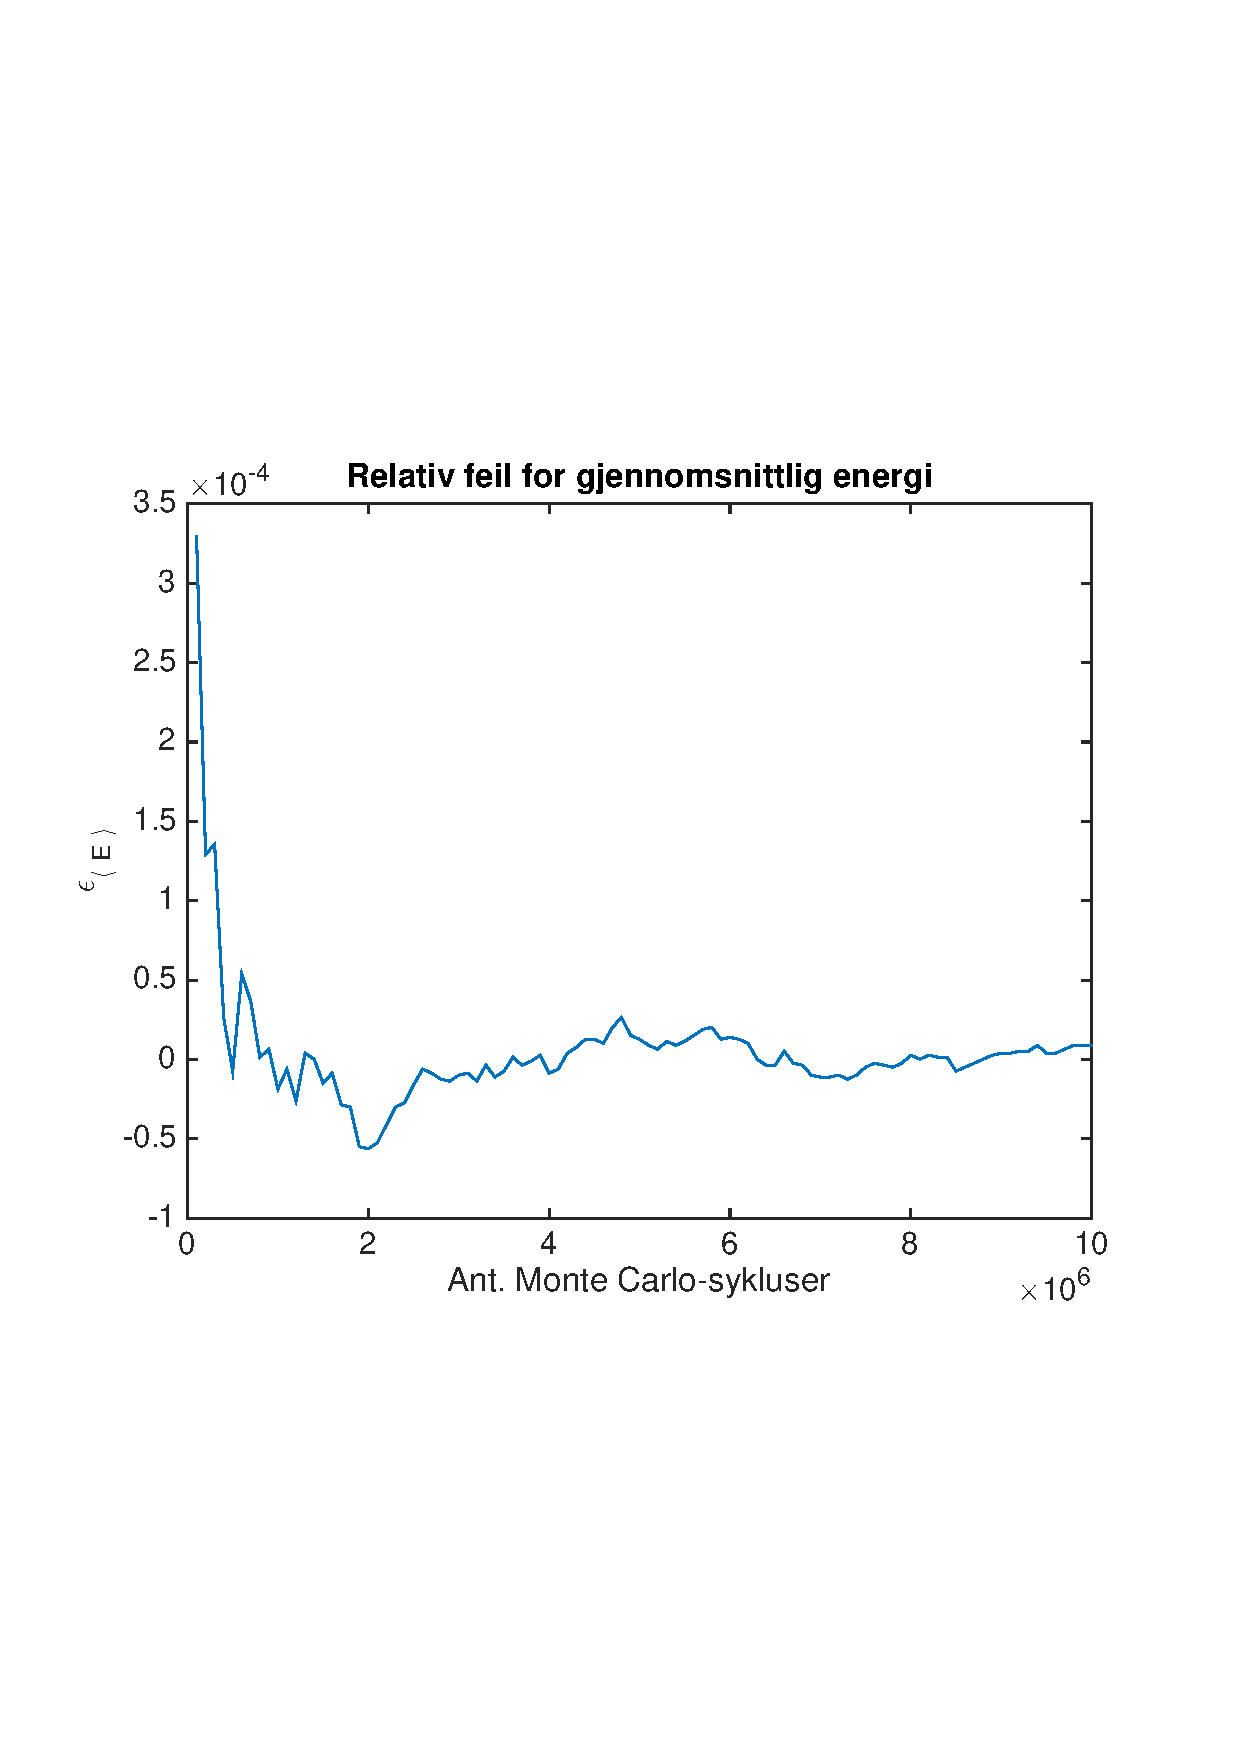
\includegraphics[scale = 0.6, trim = 1cm 8cm 1cm 8cm]{b_rel_err_avgEnergy_L2_T1.pdf}
\caption{Relativ feil for snittenergi i et $2\times2$-gitter. Vi ser at feilen aldri er spesielt stor, den er i størrelsesorden $10^{-4}$ eller mindre, noe som er akseptabelt for oss. Når systemet har nådd likevekt er feilen enda i størrelsesorden $10^{-6}$, noe som er ganske bra. Programmet ble satt til å regne ut verdiene for hver $10^4$ Monte Carlo-syklus, men ut i fra dette plottet ser det ut til at vi kunne gått mye lavere og fremdeles hatt en akseptabel relativ feil.}
\label{fig:errenergyT1L2}
\end{figure}

\begin{figure}[H]
\centering
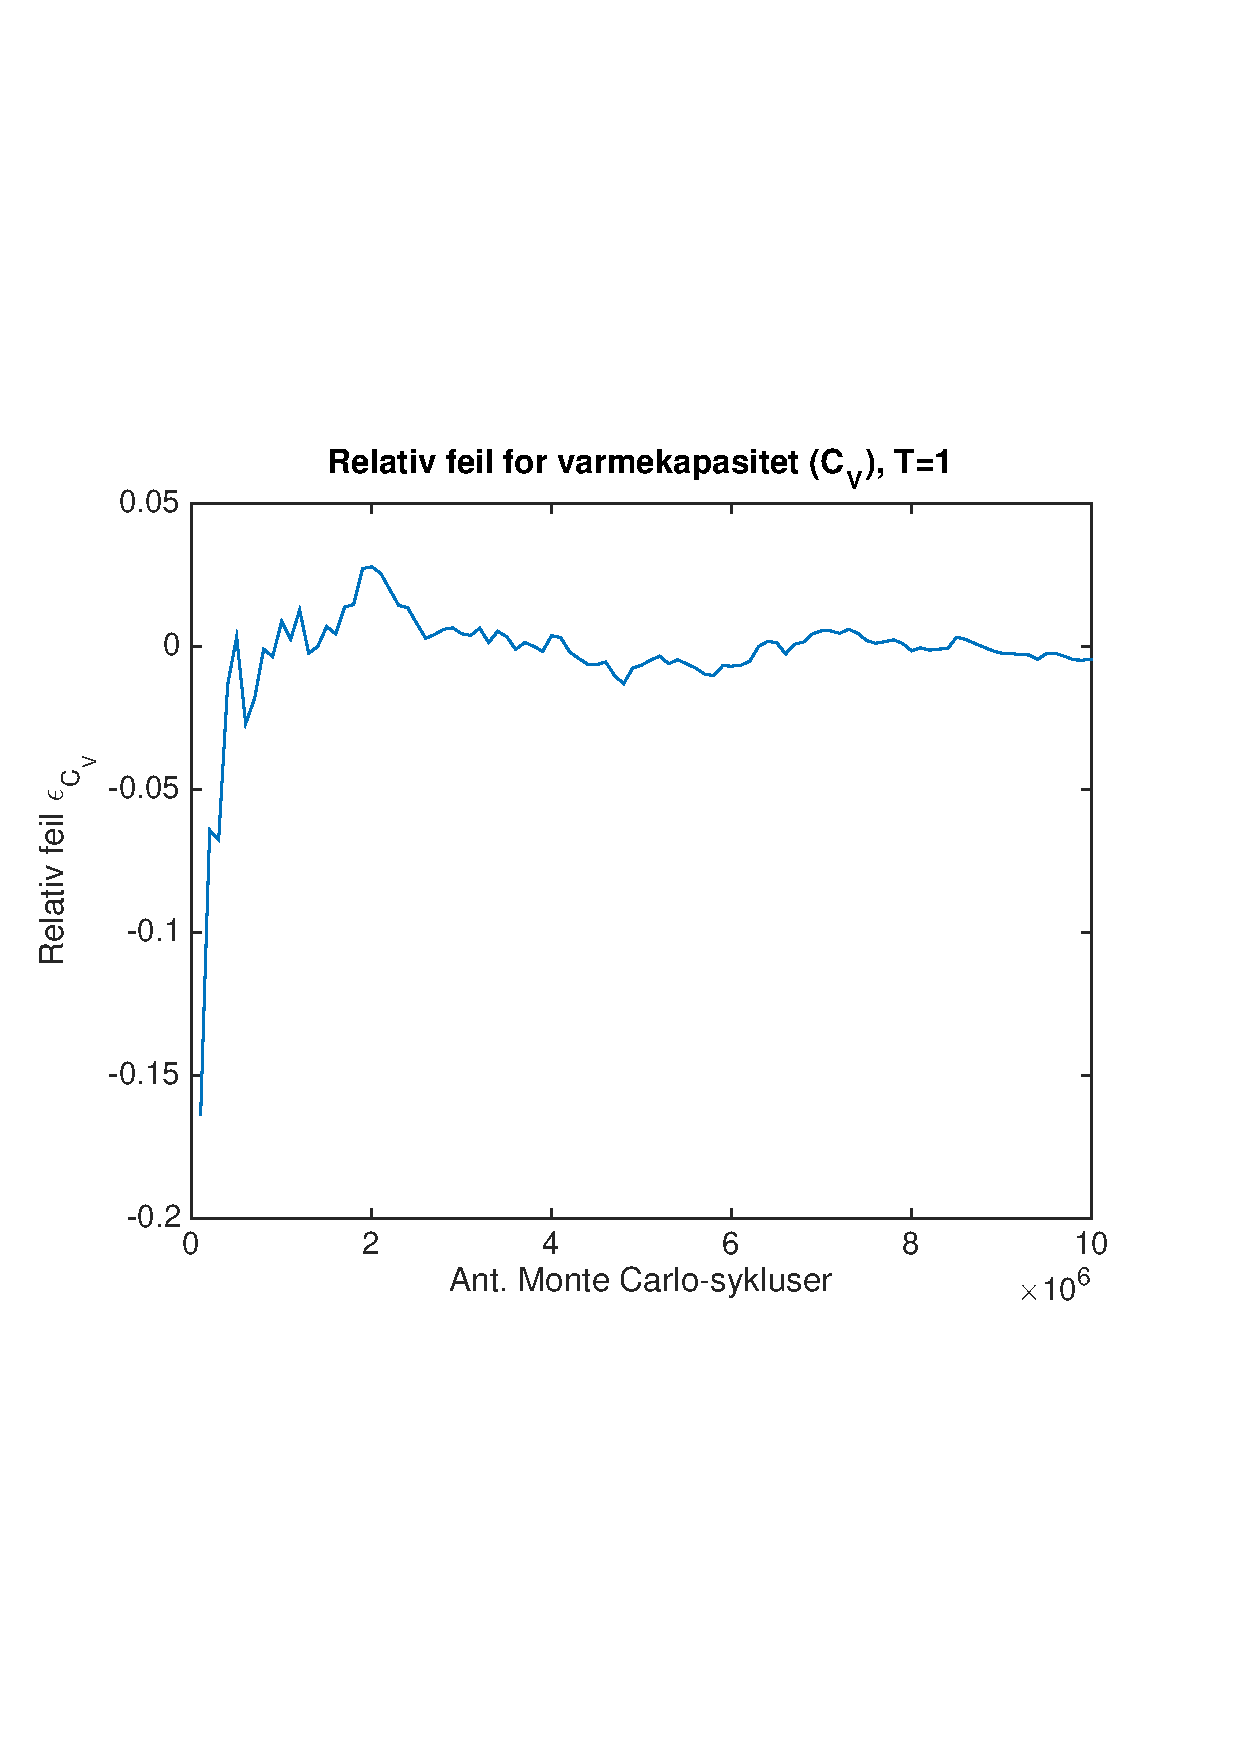
\includegraphics[scale = 0.6, trim = 1cm 8cm 1cm 8cm]{b_rel_err_c_v_L2_T1.pdf}
\caption{Her ser vi relativ feil for spesifikk varmekapasitet. Programmet bommer mest på denne i starten, og det kan være fordi temperaturen veldig lav. Se tekst for ytterligere detaljer.}
\label{fig:errcvT1L2}
\end{figure}

I fig. (\ref{fig:errcvT1L2}) så vi at den relative feilen var ganske stor i starten sammenlignet med de andre feilene. Det kommer av at temperaturen er ganske lav og at vi da får $\langle E^2 \rangle$ og $\mean{E}^2$ nesten helt like hverandre og noen små feil i programmet kan da gjøre store utslag. En feil vi hadde i programmet befant seg i \verb for -løkka for MC-syklusene. Vi hadde først satt at den skulle gå fra $n=0$ til $n\leq N_{MC}$, men da gjorde vi i realiteten $N_{MC} + 1$ MC-sykluser, noe som er greit, men problemet oppstår når vi skal normalisere verdiene i det vi regner ut $C_V$, siden normaliseringa (i funksjonen \verb ExpectationValues) da var ett siffer feil, så fikk det veldig mye å si når $T$ var lav. Vi løste problemet ved å sette løkka til å gå opp til $n < N_{MC}$.

\begin{figure}[H]
\centering
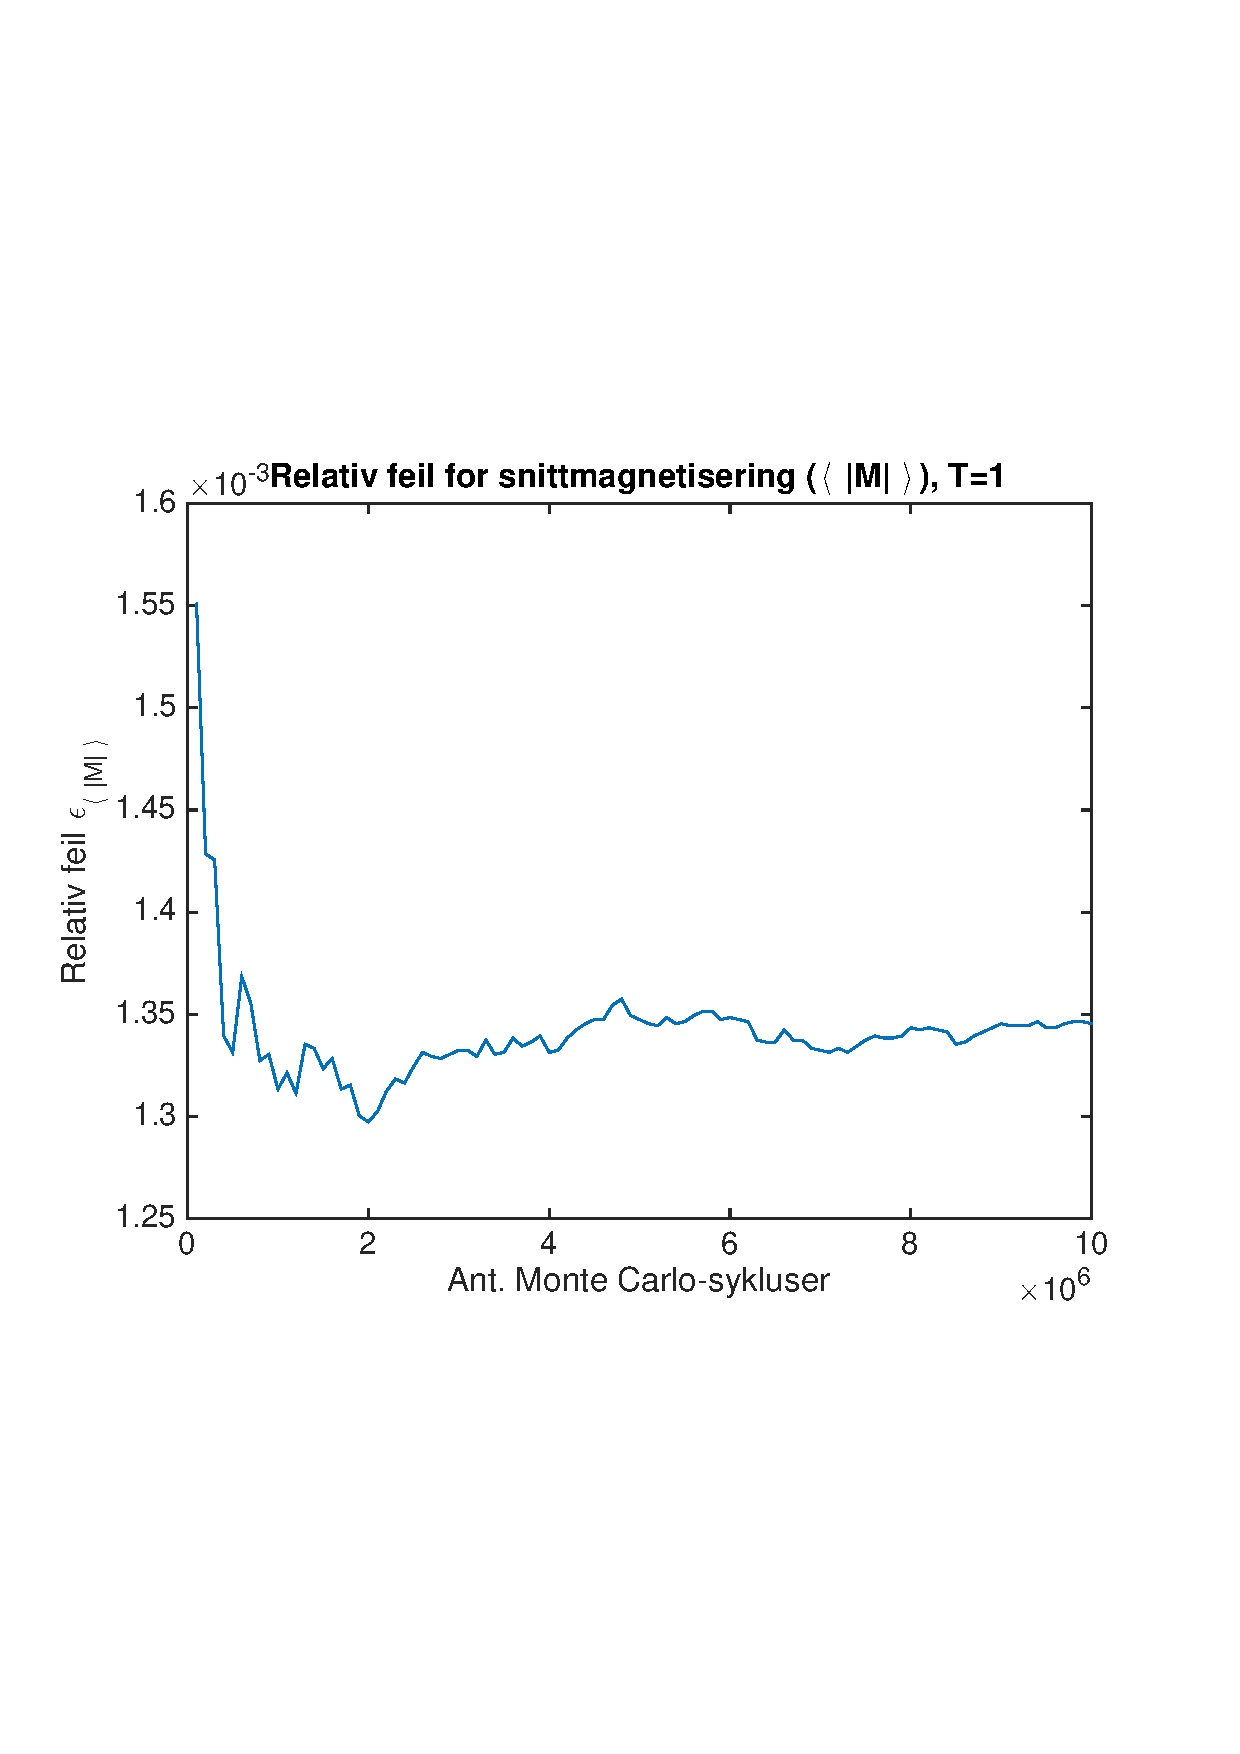
\includegraphics[scale = 0.6, trim = 1cm 8cm 1cm 8cm]{b_rel_err_mag_L2_T1.pdf}
\caption{Den relative feilen for snittmagnetisering er liten hele veien, i størrelsesorden $10^{-3}$.}
\label{fig:errmagT1L2}
\end{figure}

\begin{figure}[H]
\centering
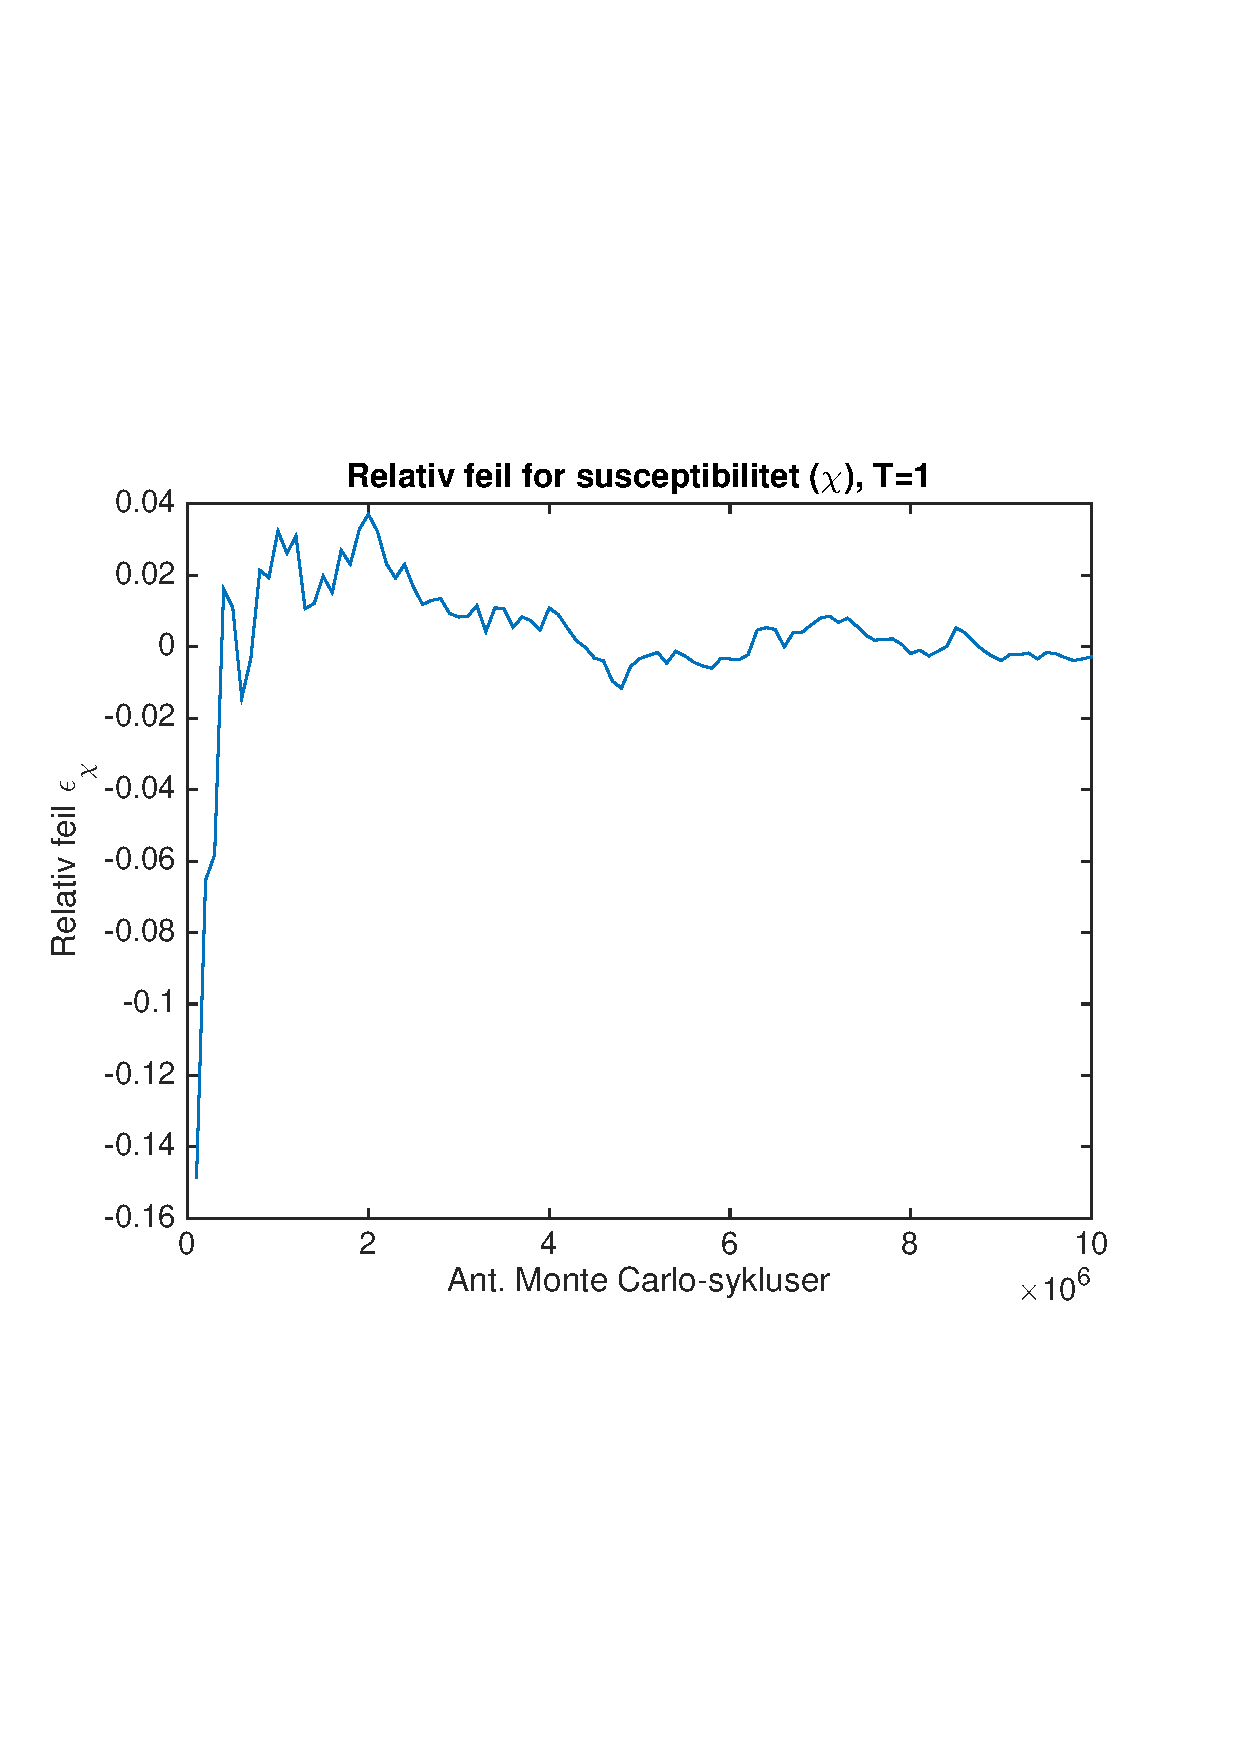
\includegraphics[scale = 0.6, trim = 1cm 8cm 1cm 8cm]{b_rel_err_chi_L2_T1.pdf}
\caption{Susceptibiliteten har også en stor relativ feil i starten, men tar seg fort inn og kommer ned i en feil på $10^{-2}$ ser det ut til.}
\label{fig:errchiT1L2}
\end{figure}


\section*{Resultat}
Vi ser først på resultatene fra ``enhetstestinga'' av programmet. Vi simulerte et gitter med $2\times2$ spinn for temperaturene $T=1$ og $T=2.4$, begge med ordnet og uordnet starttilstander. Resultatene er plottet som verdier per spinn slik at det er enkelt å sammenlikne resultater for flere gitterstørrelser. I figurene (\ref{fig:meanET1}), (\ref{fig:varmekapT1}), og (\ref{fig:chiT1}) ser vi resultatene av kjøringer med 10 millioner MC-sykluser for $T=1$. Vi ser at verdiene konvergerer raskt mot en likvektstilstand og at det ikke er nødvendig med 10 millioner MC-sykluser. Standardavvikene er ganske små, så vi kan tillate oss å gå helt ned til én million MC-sykluser når vi skal kjøre for flere temperaturer etter hverandre, som nevnt tidligere vil de påfølgende temperaturstegene ha en kort termaliseringsprosess siden vi kommer til å sette temperatursteget til $\Delta T = 0.01$.

Vi ser også at første verdien som beregnes i alle plottene treffer på første desimal eller bedre, noe som er ganske bra. Det kan se ut som om vi bommer godt på likevektstilstanden i starten, men realiteten er at programmet faktisk treffer ganske bra. La oss se nærmere på fig. (\ref{fig:meanET1}). Første beregna verdi der er $\mean E = -7.9866$, mens den analytiske verdien er $\mean E = -7.9839$, noe som gir en relativ feil på $\epsilon = 0.3296 \cdot 10^{-3}$, som vi tør påstå er ganske bra.

\begin{figure}[H]
\centering
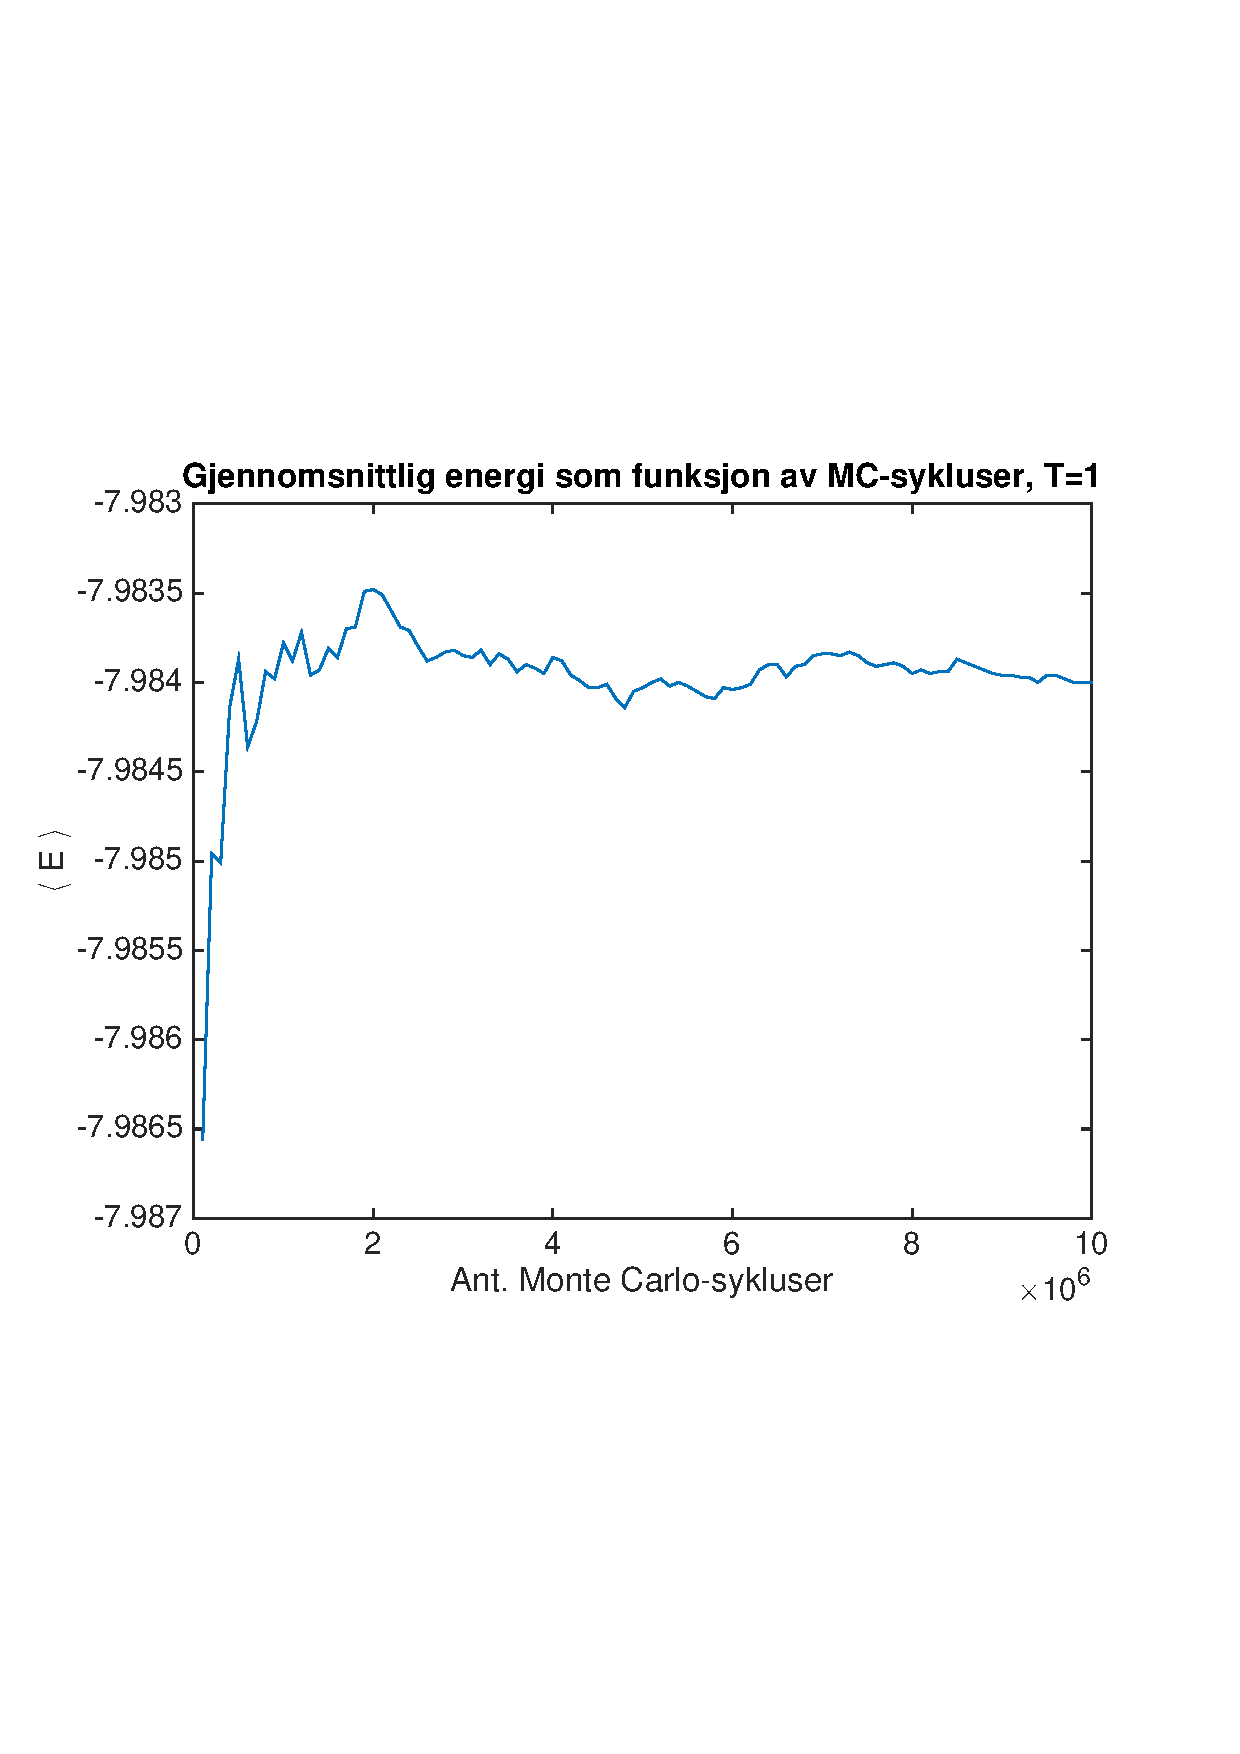
\includegraphics[scale = 0.6, trim = 1cm 8cm 1cm 8cm]{b_avgEnergy_MC_L2_T1.pdf}
\caption{Her er $\mean E$ plottet som funksjon av antall MC-sykluser for ordnet og uordnet starttilstand. Vi ser at første verdi for snittenergien er ganske bra, den treffer på andre desimal, og tar seg raskt inn til likevektstilstanden. Det vil ikke være noe problem å se bort i fra termaliseringsprosessen så lenge vi kjører en million sykluser.}
\label{fig:meanET1}
\end{figure}

\begin{figure}[H]
\centering
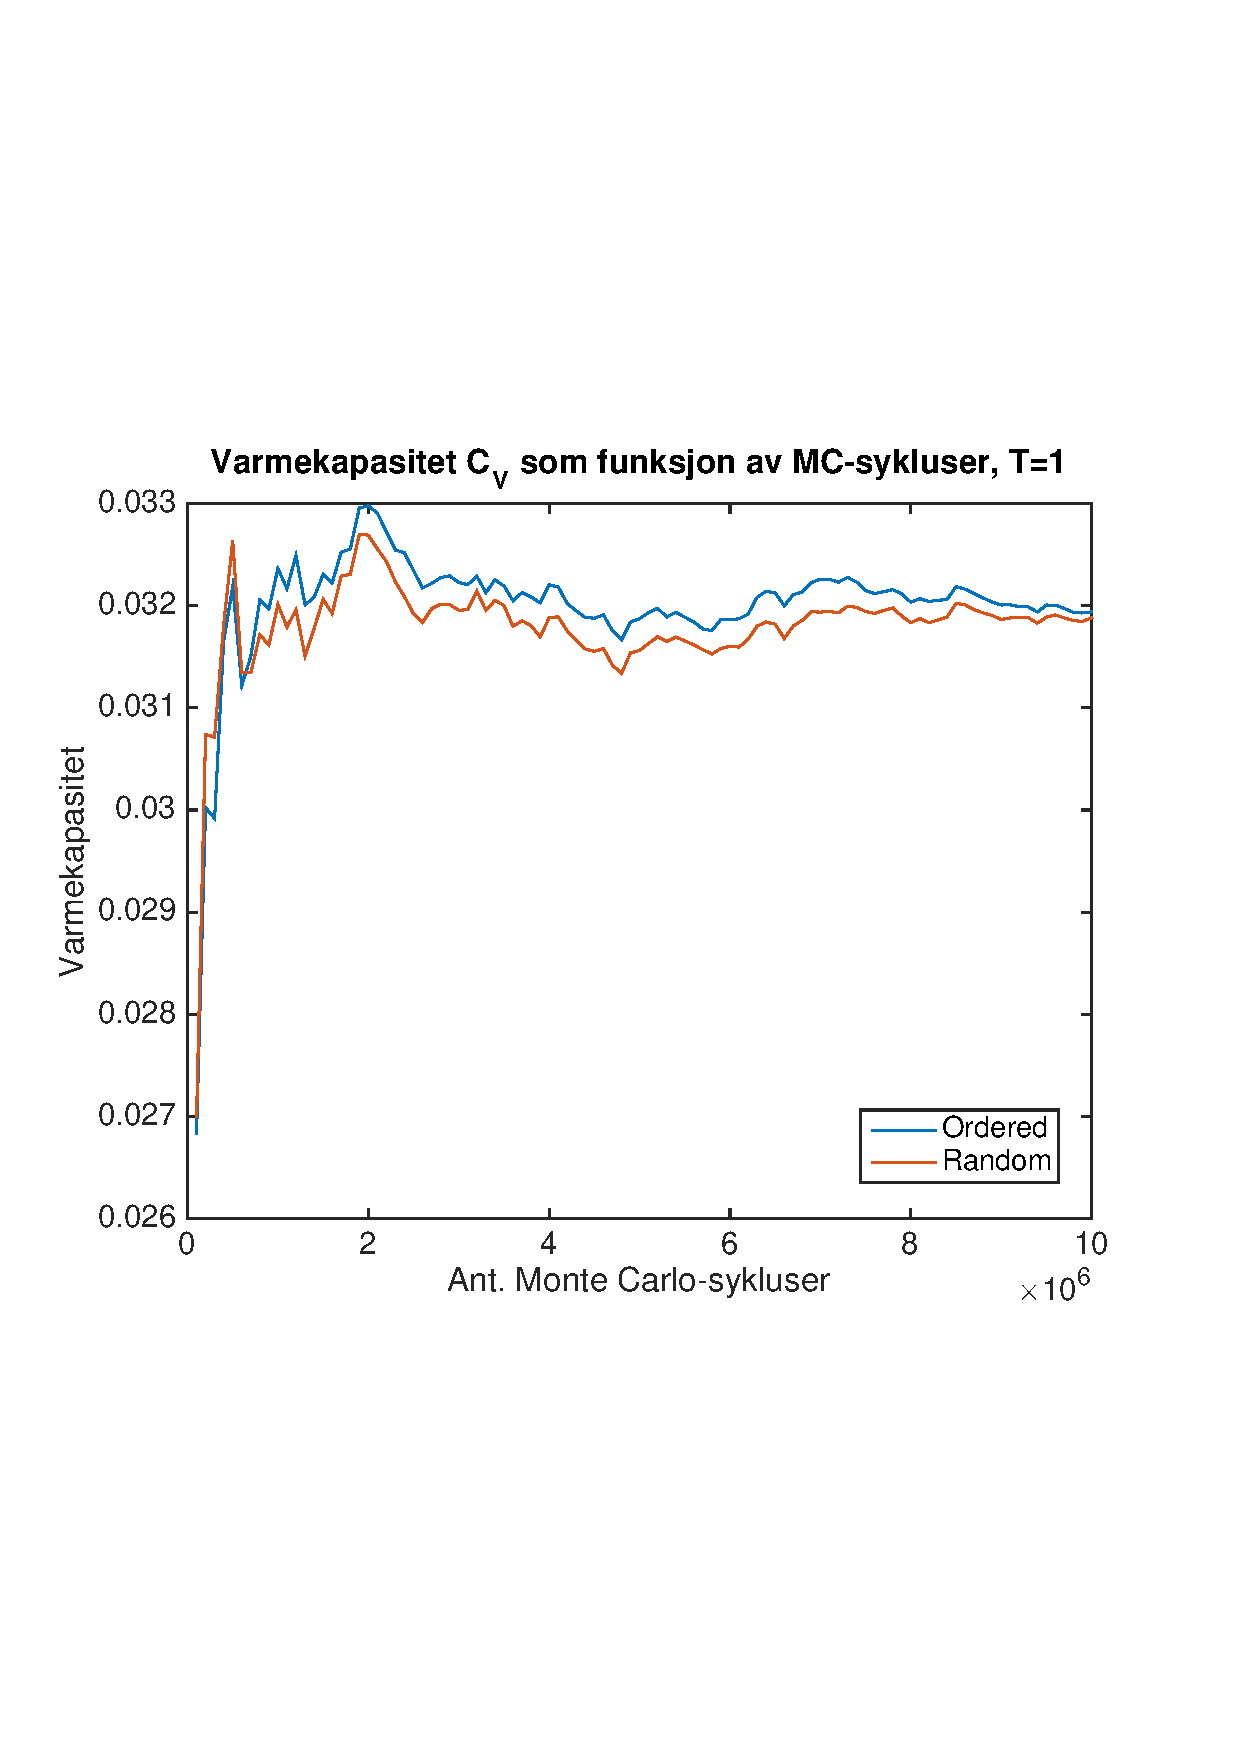
\includegraphics[scale = 0.6, trim = 1cm 8cm 1cm 8cm]{b_varmekap_MC_L2_T1.pdf}
\caption{Vi ser at varmekapasiteten blir estimert litt dårligere i starten enn snittenergien ble, slik vi også så i numerisk presisjon-seksjonen ovenfor.}
\label{fig:varmekapT1}
\end{figure}

\begin{figure}[H]
\centering
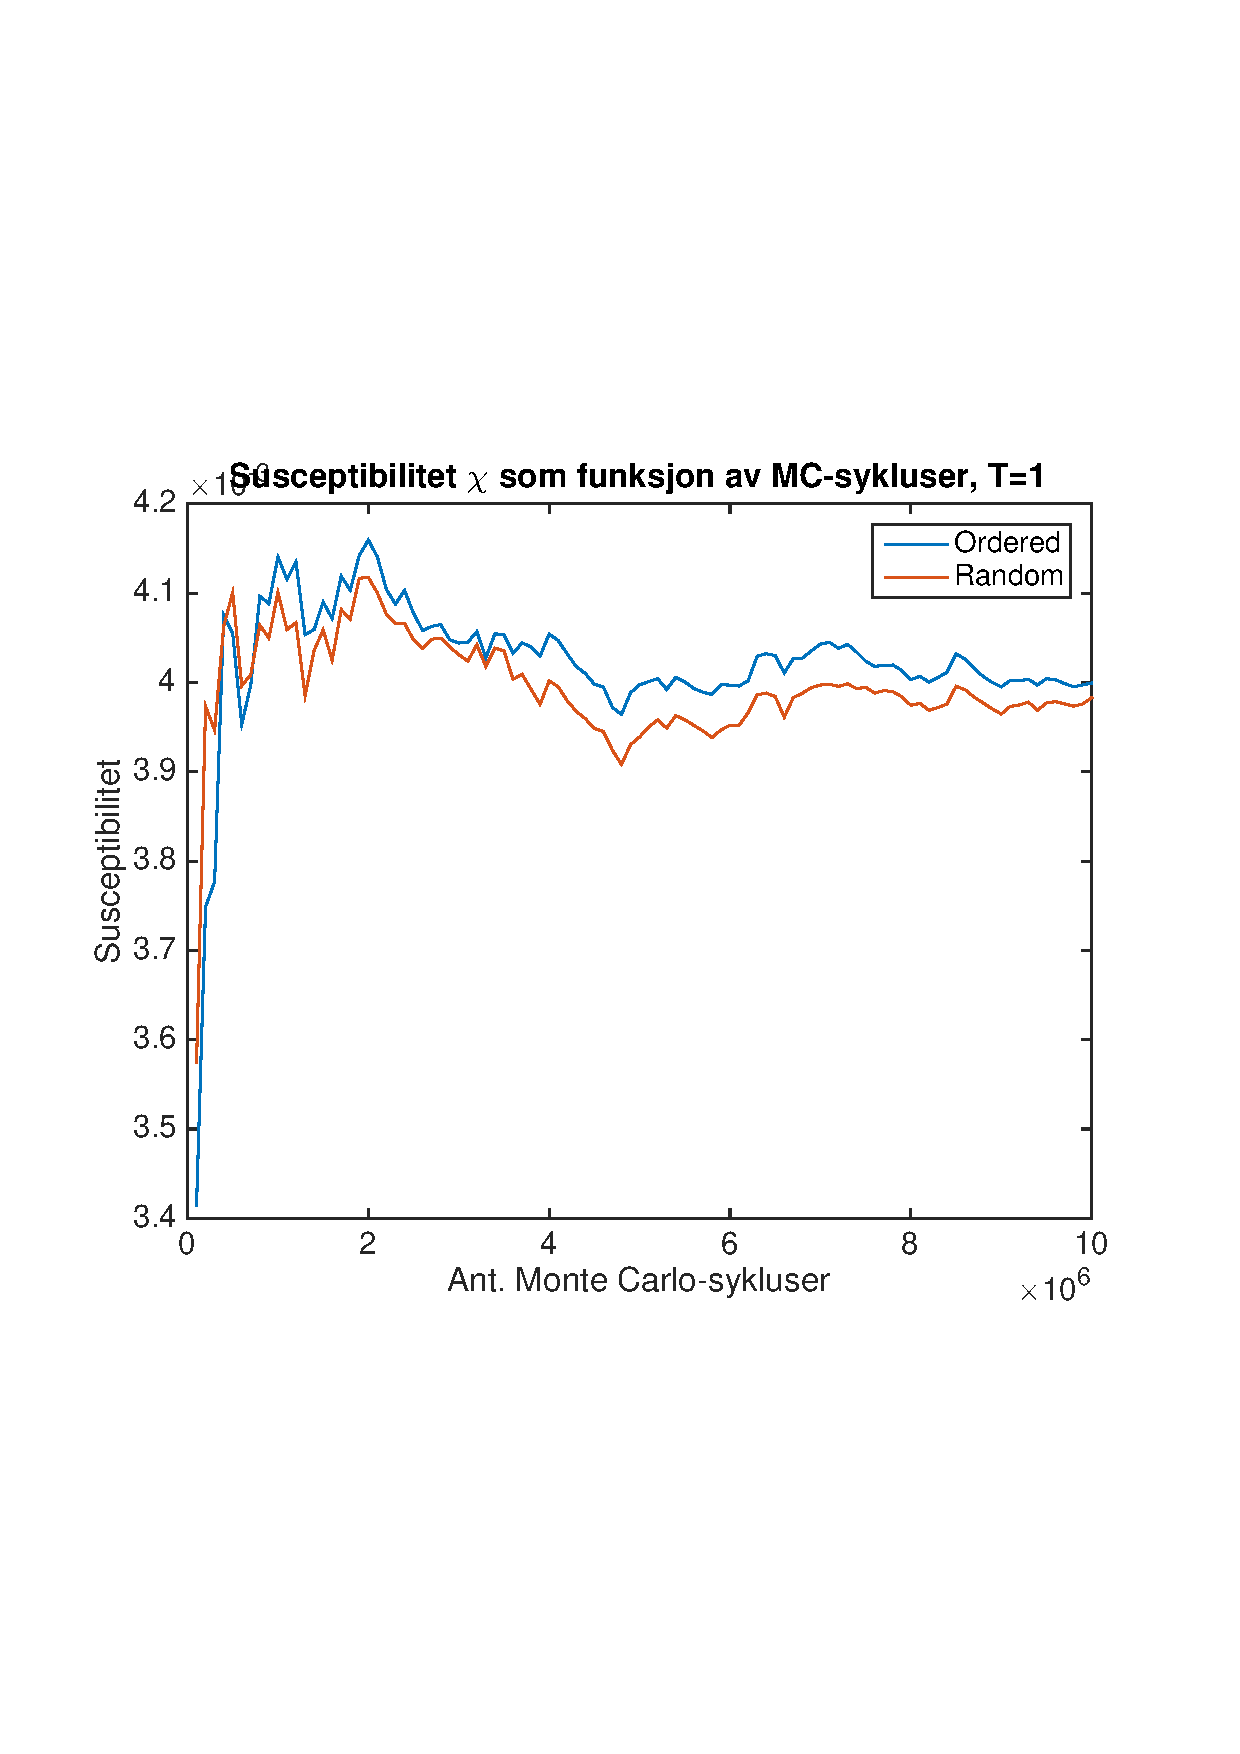
\includegraphics[scale = 0.6, trim = 1cm 8cm 1cm 8cm]{b_chi_MC_L2_T1.pdf}
\caption{I forrige seksjon fant vi at beregnet verdi for susceptibiliteten bommet litt i starten, men tok seg fint inn, vi ser det samme her også. Vi legger også merke til at starttilstanden har litt å si for hvilken verdi likevektstilstanden tar, den ordnete starttilstanden legger seg på en litt høyere susceptibilitet enn den uordnete.}
\label{fig:chiT1}
\end{figure}

Vi kan så øke temperaturen til $T=2.4$ og se hvordan forskjellene mellom ordnet uordnet starttilstand er da. I figurene (\ref{fig:meanET24}), (\ref{fig:varmekapT24}), og (\ref{fig:chiT24}) ser vi resultatene. Vi ser at grafene ligger helt oppå hverandre, i noe de ikke gjorde for $T=1$.

For $T=2.4$ har vi ikke regnet ut relativ feil, men vi kan se på hvor mange desimaler unna første beregnet verdi er fra likevektsverdien. Snittenergien treffer på andre desimal, varmekapasitet på første desimal, og ditto med susceptibilitet. Vi kan også merke oss at for $T=2.4$ så ser det ut til at systemet gjør litt større svingninger enn for $T=1$ før det når likevektstilstanden.

\begin{figure}[H]
\centering
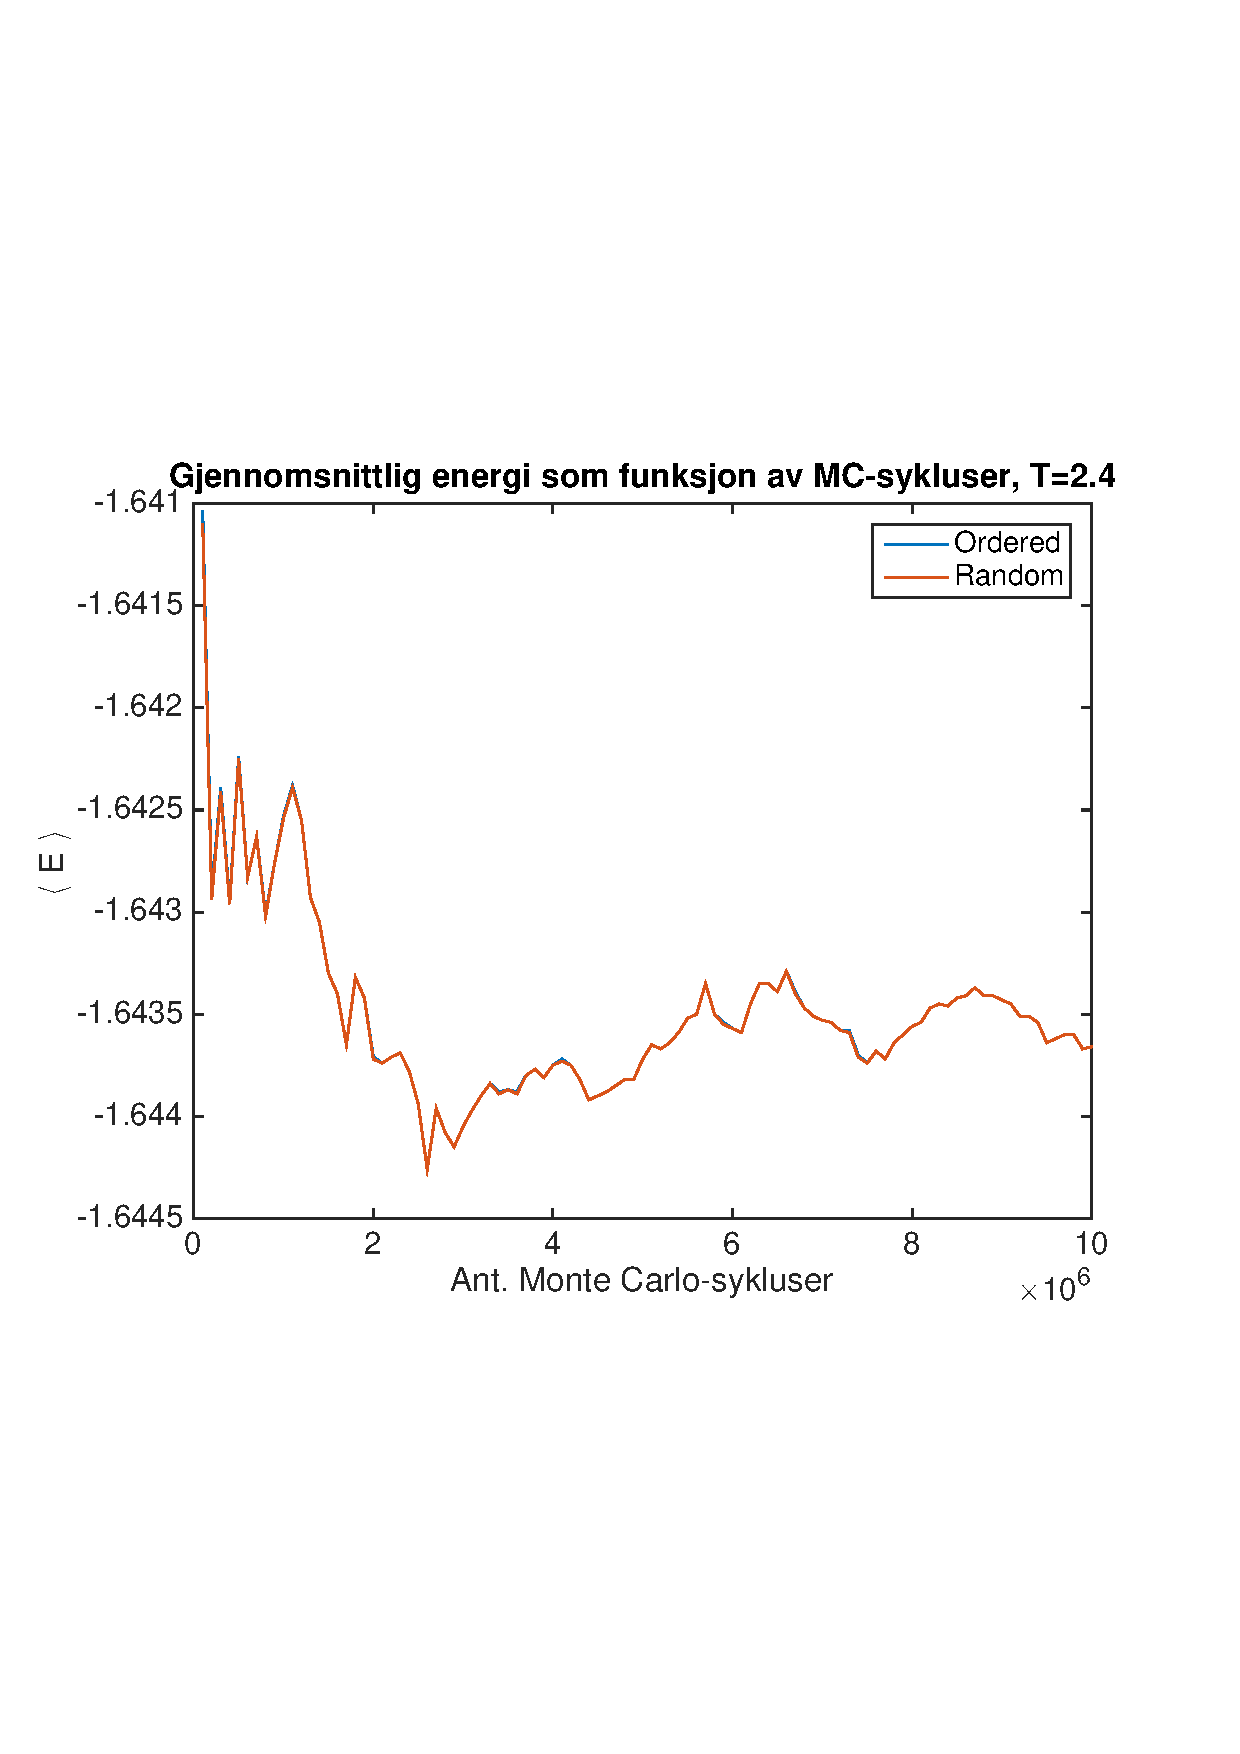
\includegraphics[scale = 0.6, trim = 1cm 8cm 1cm 8cm]{b_avgEnergy_MC_L2_T24.pdf}
\caption{Her er $\mean E$ plottet som funksjon av antall MC-sykluser for ordnet og uordnet starttilstand. Vi ser at første verdi for snittenergien er ganske bra, den treffer på andre desimal, og tar seg raskt inn til likevektstilstanden.}
\label{fig:meanET24}
\end{figure}

\begin{figure}[H]
\centering
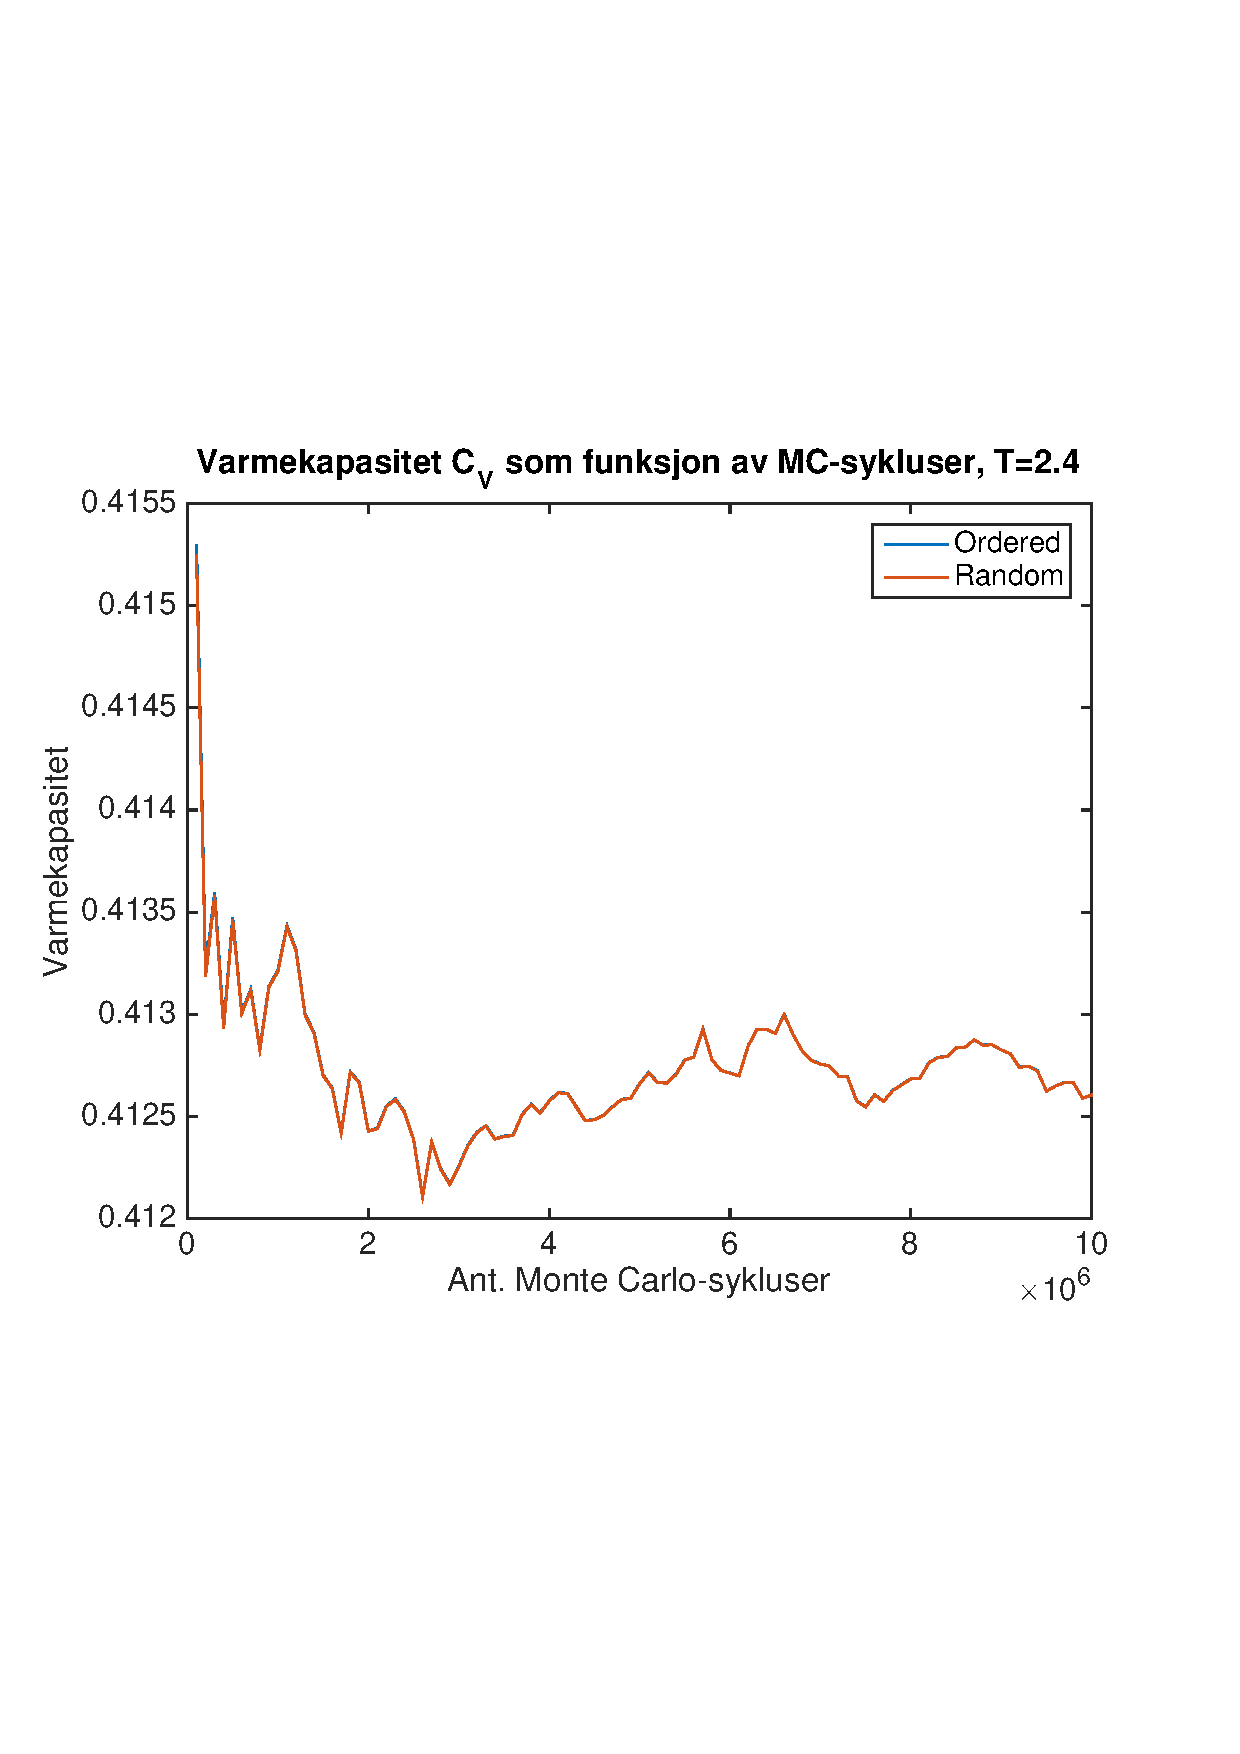
\includegraphics[scale = 0.6, trim = 1cm 8cm 1cm 8cm]{b_varmekap_MC_L2_T24.pdf}
\caption{Vi ser at varmekapasiteten blir estimert litt dårligere i starten enn snittenergien ble, men standardavviket er $\sigma_{C_V} = 3.6538\cdot10^{-4}$. Vi kan altså se bort fra termaliseringa her også.}
\label{fig:varmekapT24}
\end{figure}

\begin{figure}[H]
\centering
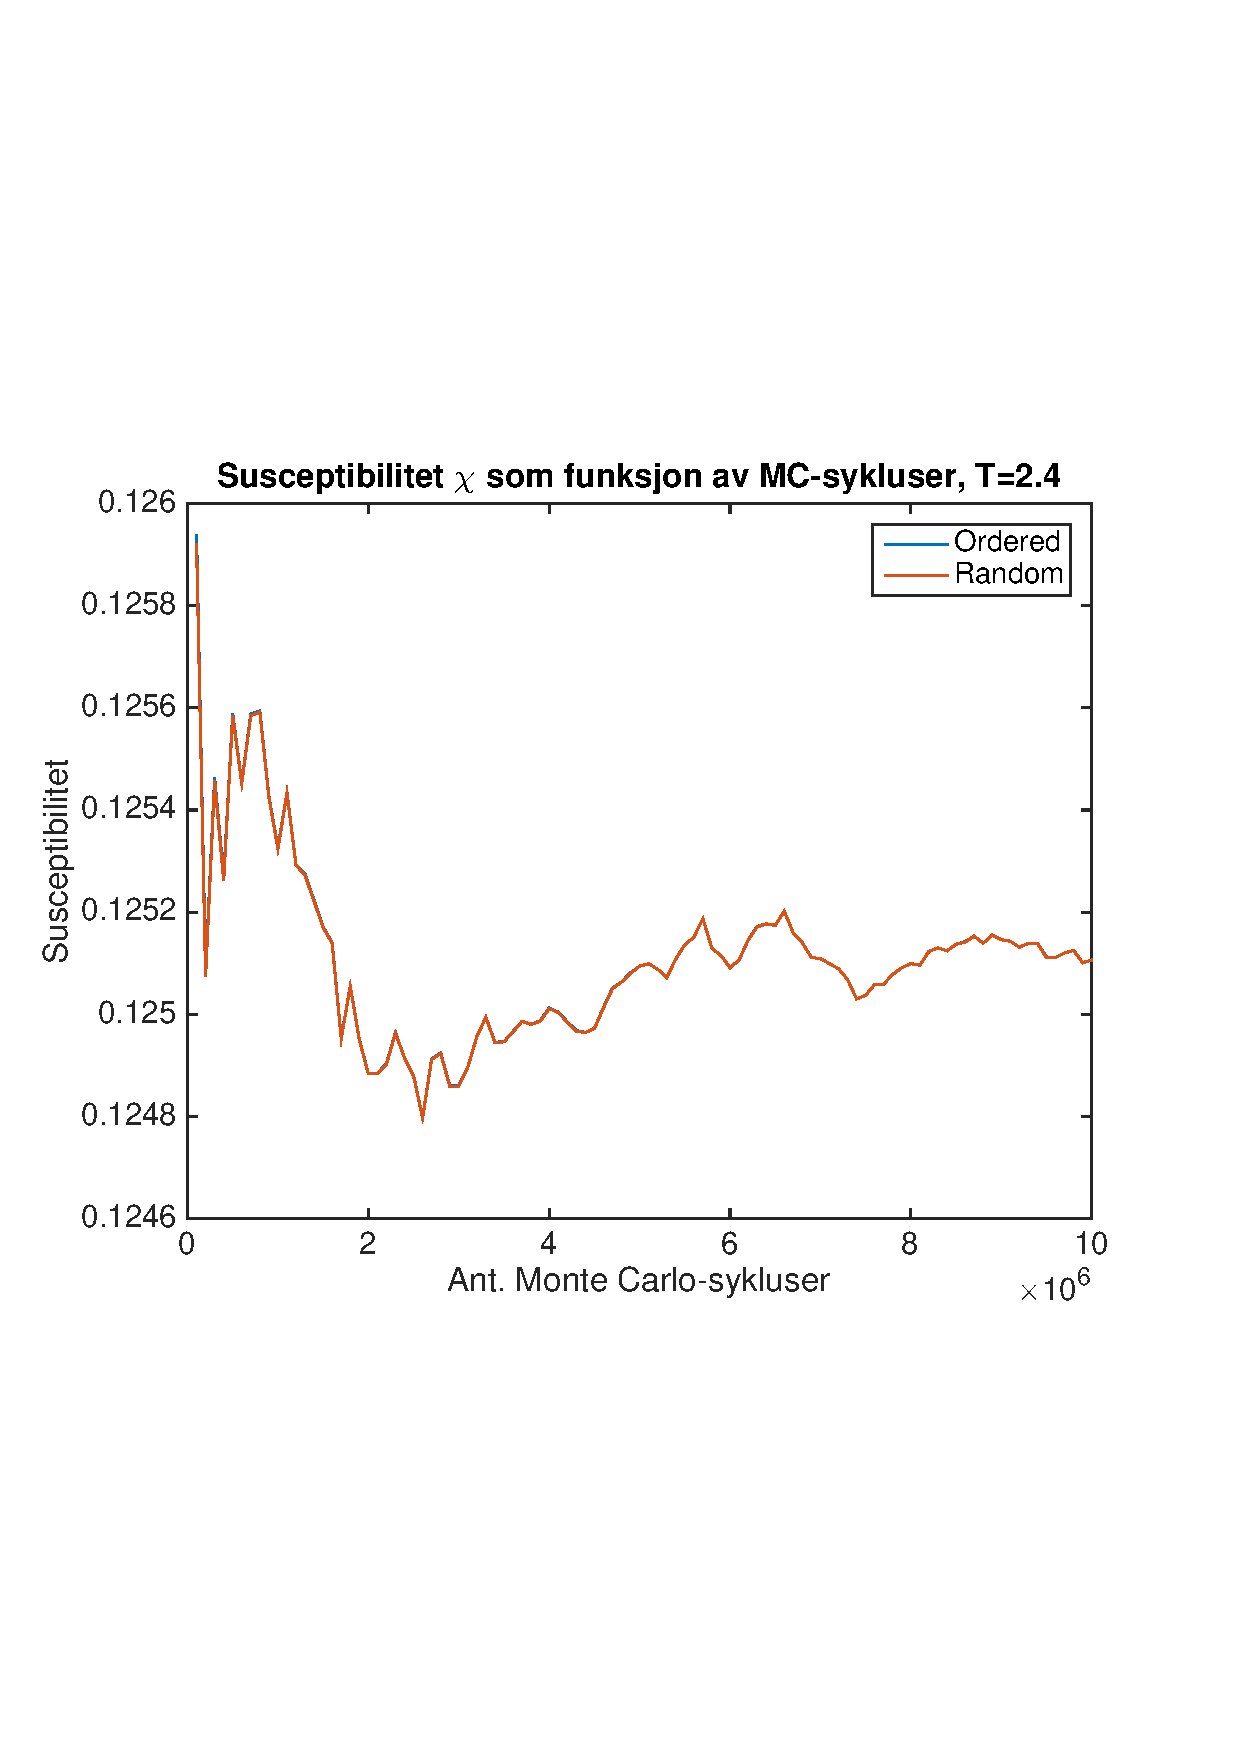
\includegraphics[scale = 0.6, trim = 1cm 8cm 1cm 8cm]{b_chi_MC_L2_T24.pdf}
\caption{Susceptibiliteten får et estimat som er et stykke unna likevektsverdien, men etter to millioner MC-sykluser er den så å si i likevekt.}
\label{fig:chiT24}
\end{figure}

Vi kan så ta en titt på fordelinga av energitilstander. I fig. (\ref{fig:histT24}) så ser vi histogrammet over energitilstander etter å ha oppnådd likevekt. Histogrammet sentrerer seg omkring $-500$. Vi har samlet opp data for hver 10000 MC-syklus, men det ville kanskje vært bedre å gjort det oftere slik at vi hadde fått mer data å se på.

I fig. (\ref{fig:histT1}) ser vi histogrammet for $T=1$, ikke overraskende er nesten alle tilstandene i spinn ned, altså de har verdi $-1$.
 variance_E_T24 =

    1.4010


e_var_24 =

    1.3955


variance_E_T1 =

    0.0244


e_var_1 =

    0.0235

\begin{figure}[H]
	\centering
	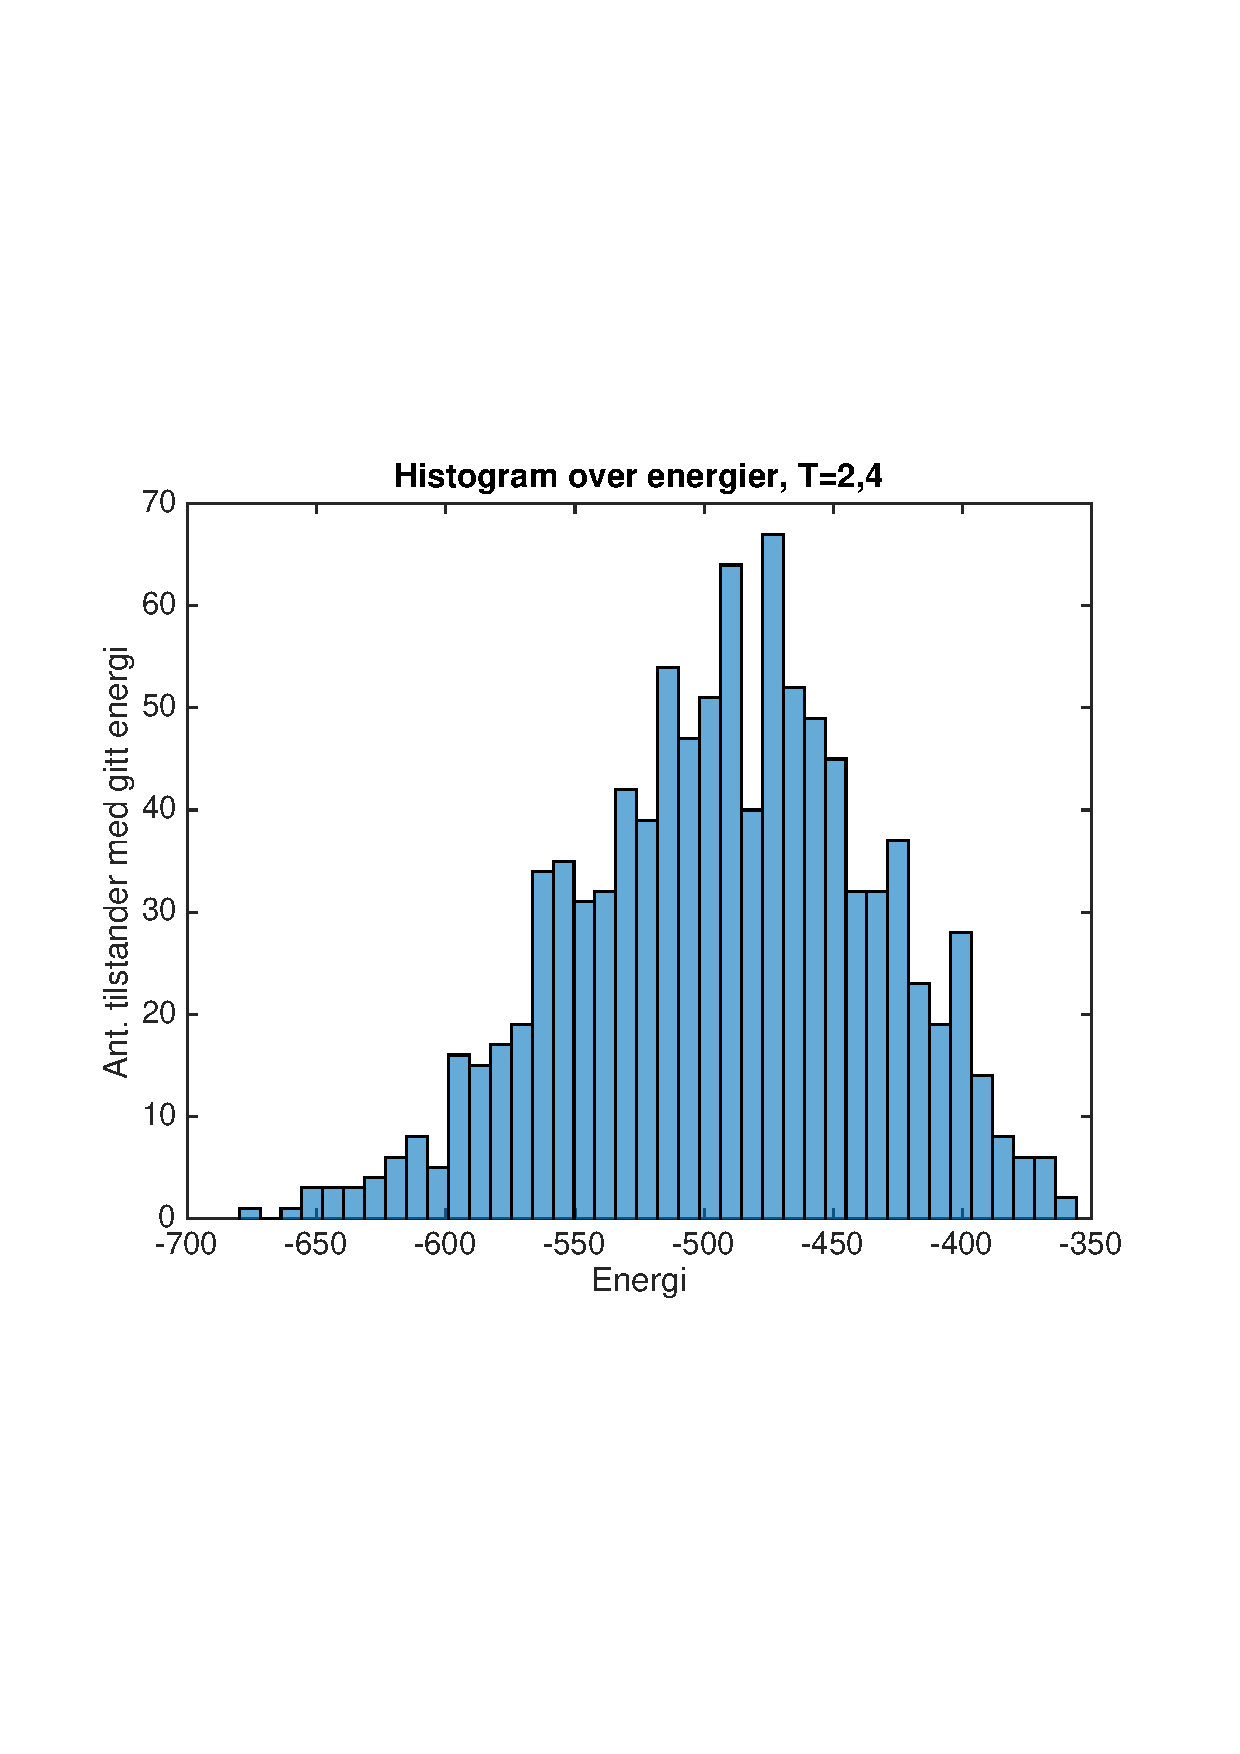
\includegraphics[scale = 0.6, trim = 1cm 8cm 1cm 8cm]{histogram_T24_L20.pdf}
	\caption{Vi ser her histogrammet som viser oss hvor ofte vi ser tilstander med visse energier for $T=2.4$. Fordelinga nærmer seg en gaussisk fordeling, for større gitter enn her vil fordelinga nok bli enda glatter.}
	\label{fig:histT24}
\end{figure}

\begin{figure}[H]
	\centering
	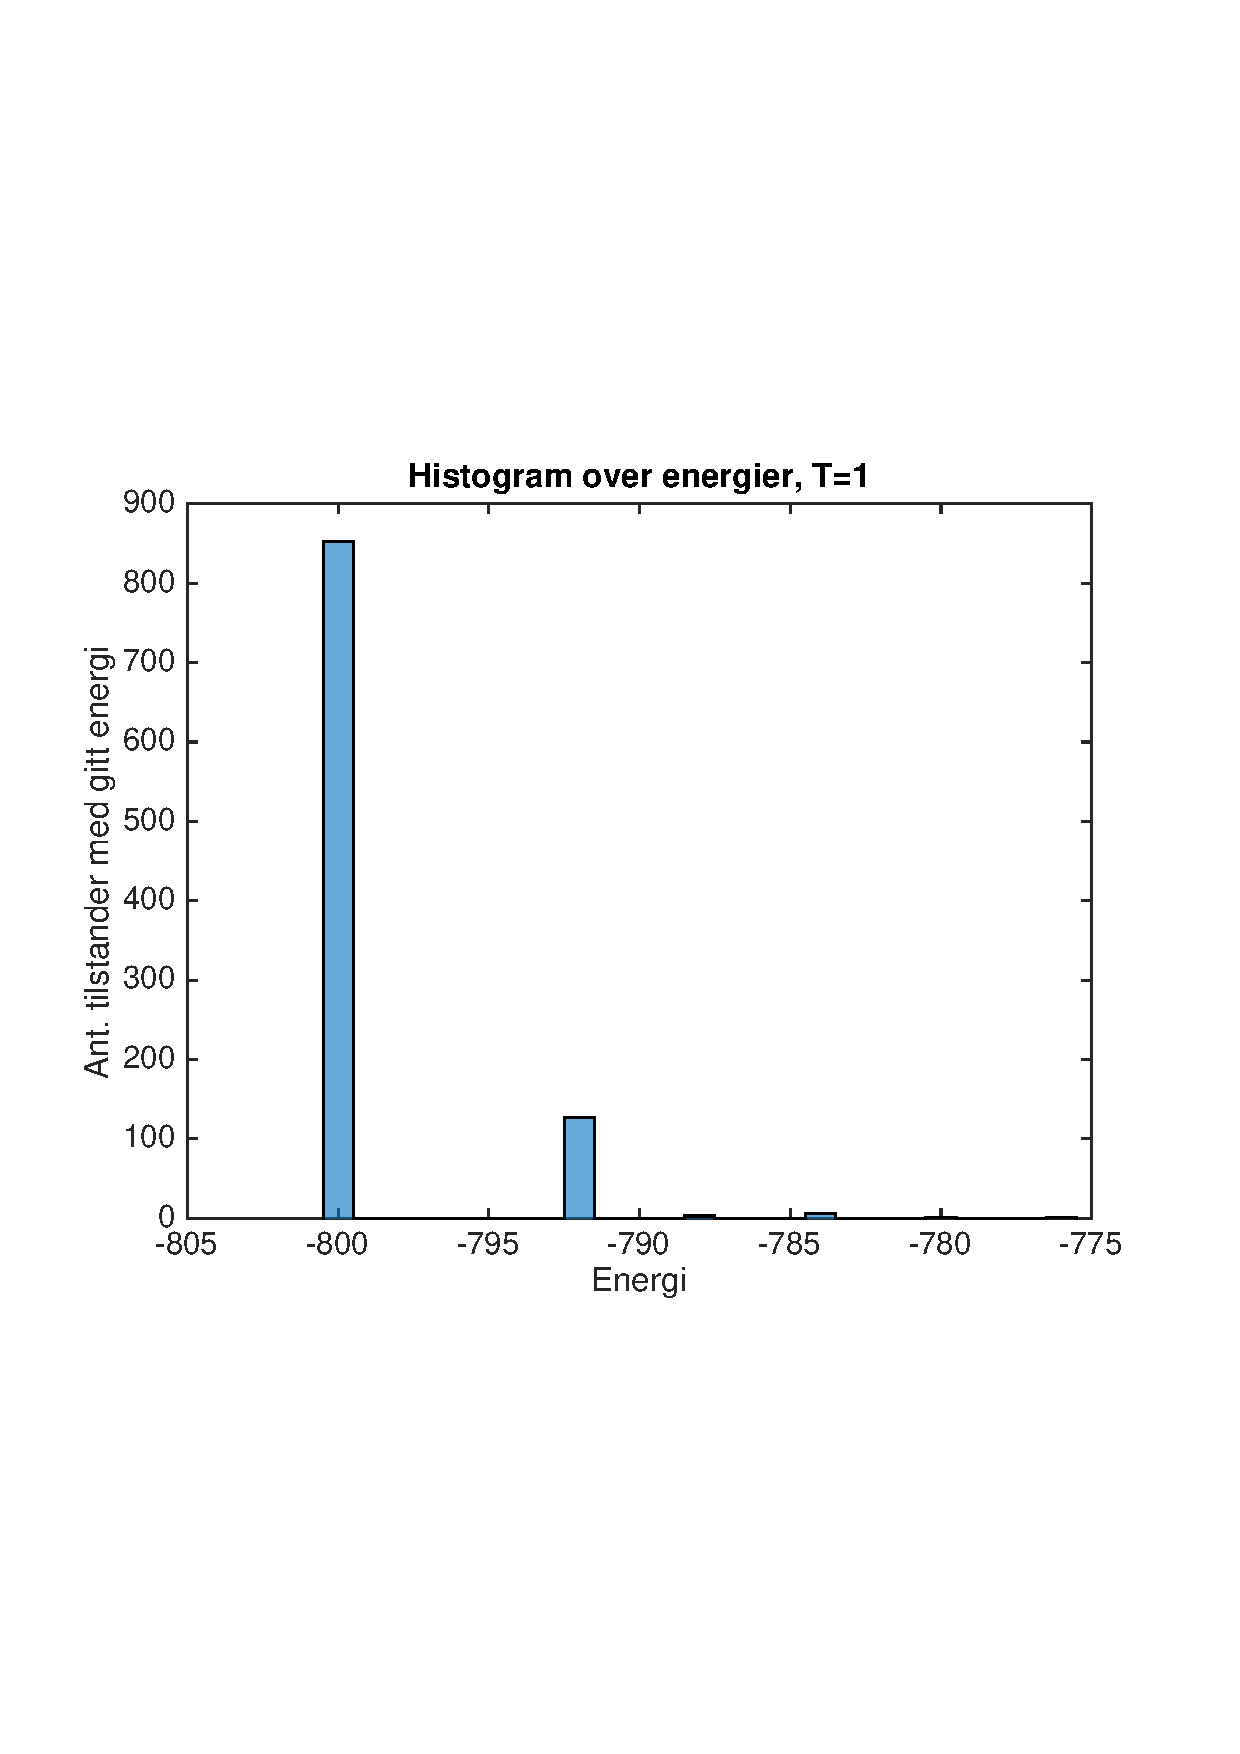
\includegraphics[scale = 0.6, trim = 1cm 8cm 1cm 8cm]{histogram_T1_L20.pdf}
	\caption{For $T=1$ ser vi at nesten alle tilstander har alle spinnene sine vendt ned. Dette er tilstanden som gir lavest energi, og siden temperatur og energi er to sider av samme sak, så vil systemet ha den laveste energien.}
	\label{fig:histT1L20}
\end{figure}

Nå har vi blitt såpass godt kjent med systemet at vi kan bruke det vi vet til å bestemme oss for antall MC-sykluser og temperatursteg slik at vi kan regne ut spesifikk varmekapasitet og  susceptibilitet til å estimere en verdi for den kritiske temperaturen $T_C$. Vi har kjørt med én million MC-sykluser og temperatursteg $\Delta T = 0.01$ for alle gitterstørrelser, $L=[20,40,60,80,100]$.

Resultatene ser vi i fig. (\ref{fig:cv_difftemp}) og (\ref{fig:chi_difftemp}). Vi ser klart og tydelig at \emph{noe} foregår rundt $T\approx 2.3$. Dette er faseovergangen vi skal se etter. Det er kanskje naturlig å tenke seg at det er lurt å bruke data fra $\chi_{num}$ til å finne et estimat for $T_C$, men det er faktisk litt lurere å bruke $C_{V,num}$ som datagrunnlag. Grunnen til det er at grafen for $\chi_{num}$ blir veldig spiss og datapunktene kan derfor sprike litt mye når vi skal finne toppunktene, valget av temperatursteg vil spille en veldig stor rolle og velger man ``galt'' så kan estimatet bli dårlig. Bruker vi derimot $C_{V,num}$ så vil toppunktet ikke ligge langt over resten av punktene og vi får et mer stabilt resultat.

\begin{figure}[H]
	\centering
	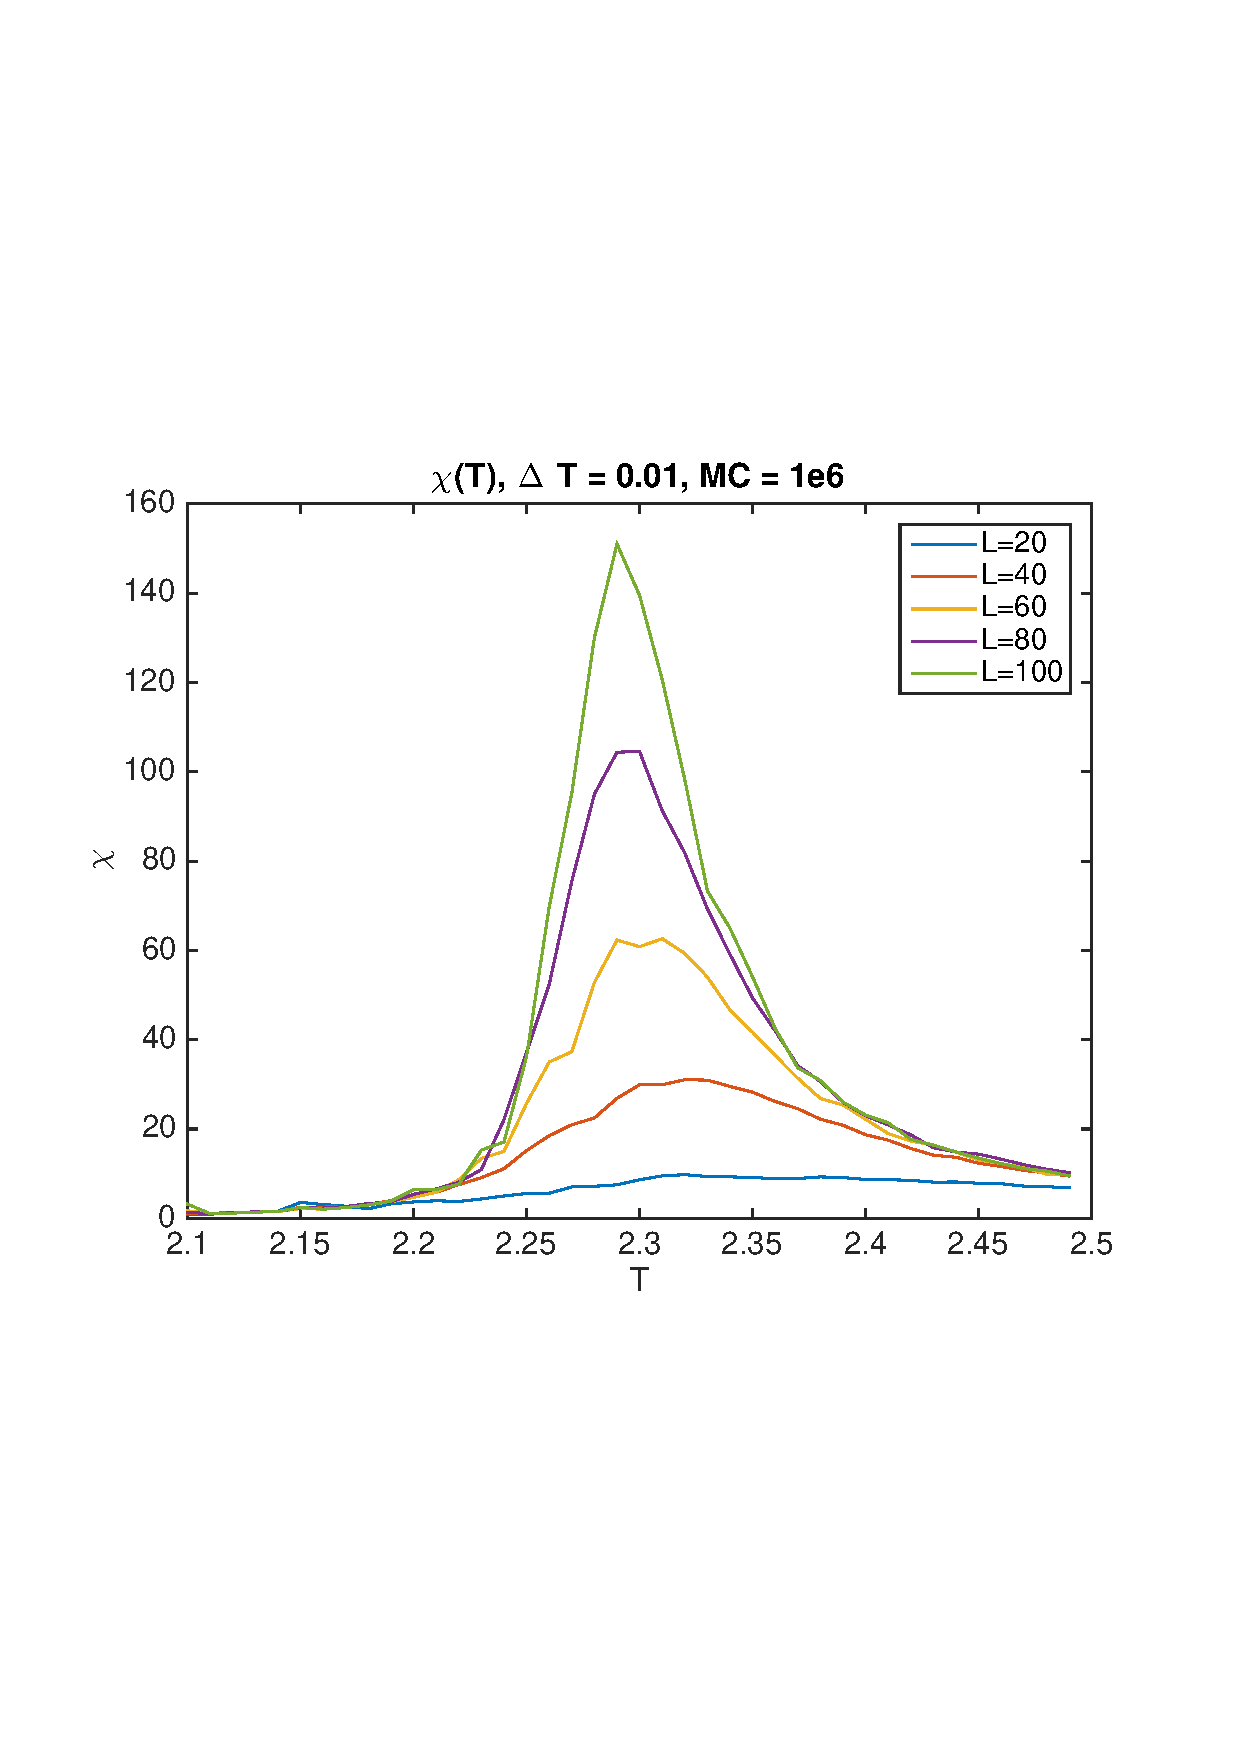
\includegraphics[scale = 0.6, trim = 1cm 8cm 1cm 8cm]{chi_difftemp.pdf}
	\caption{Her har vi plottet susceptibiliteten som funksjon av temperatur for flere gitterstørrelser. Vi ser klart at det skjer noe for $T\approx 2.3$. Dette noe er en faseovergang, i fig. (\ref{}) ser vi et estimat for faseovergangstemperaturen.}
	\label{fig:chi_difftemp}
\end{figure}

\begin{figure}[H]
	\centering
	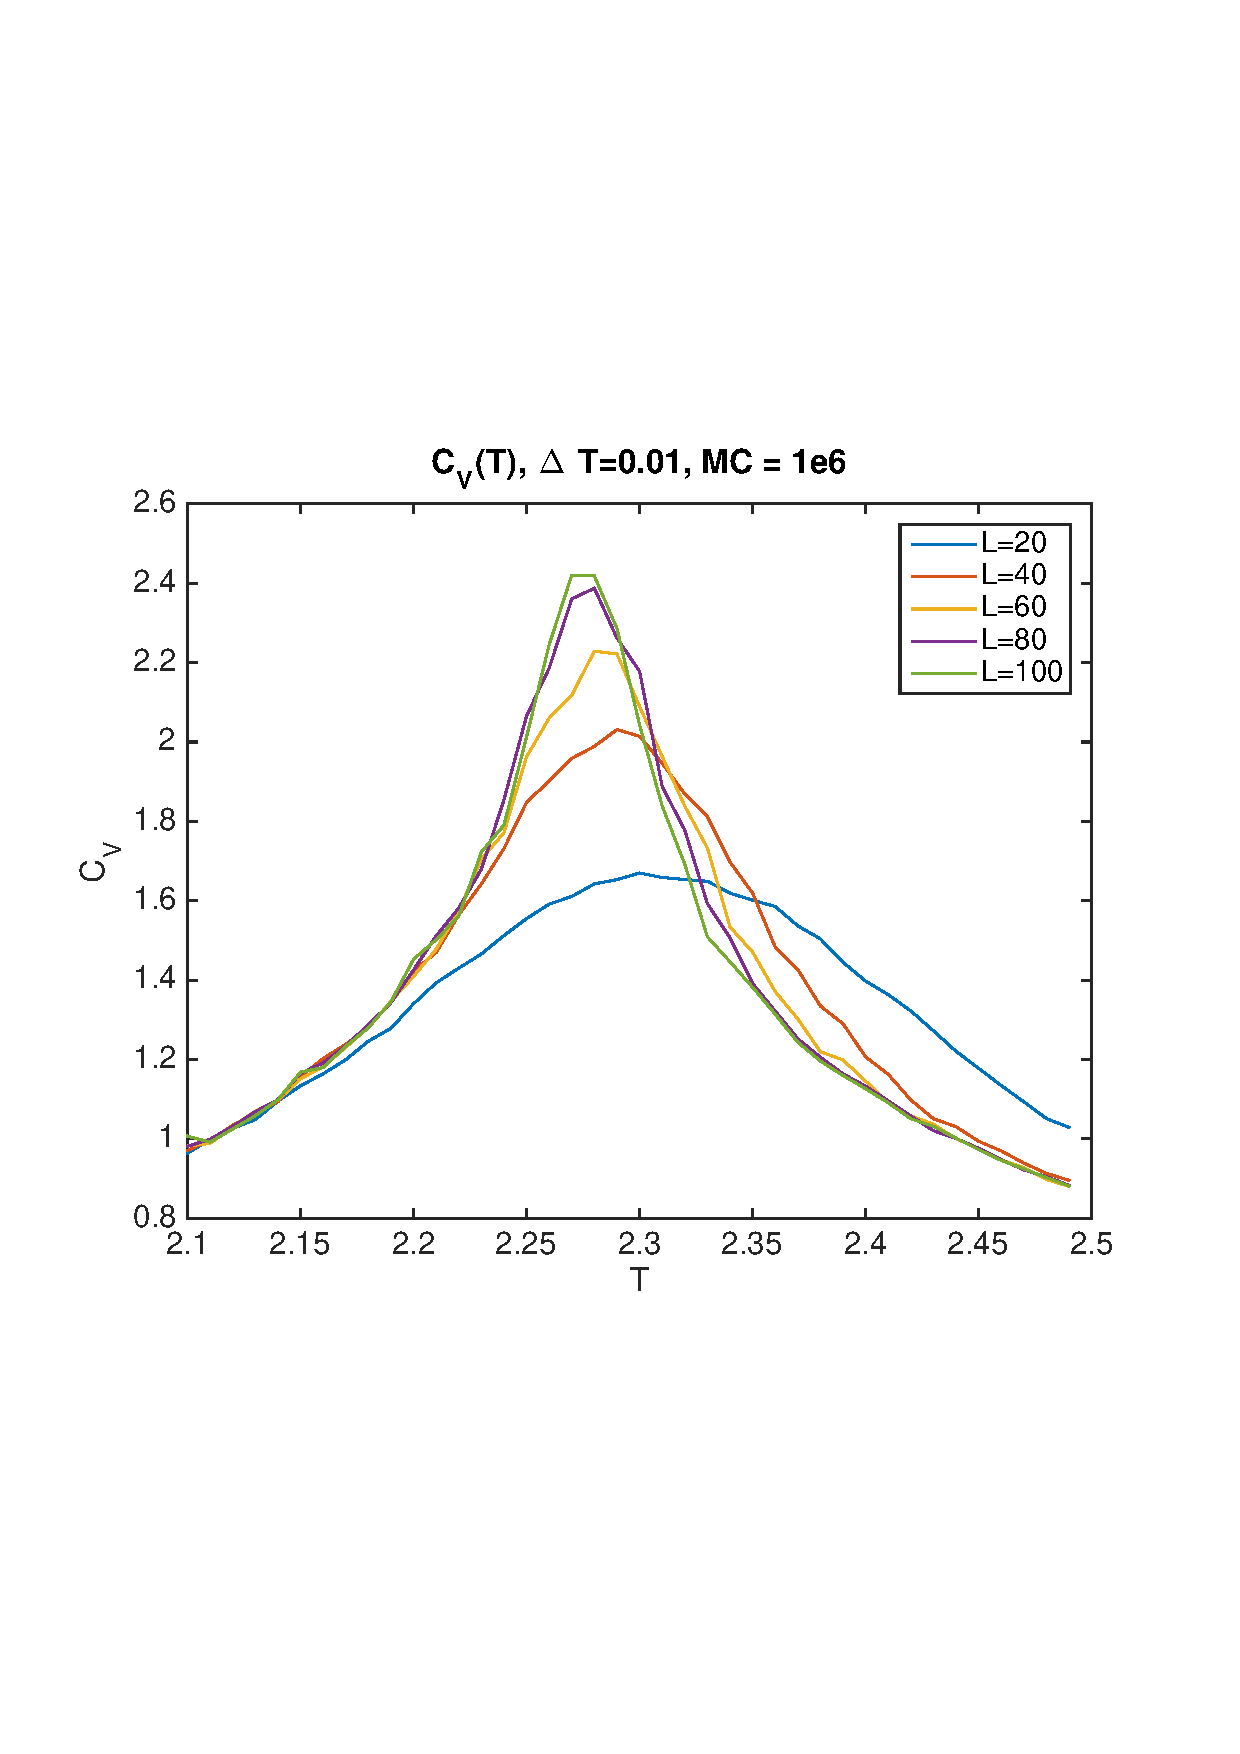
\includegraphics[scale = 0.6, trim = 1cm 8cm 1cm 8cm]{cv_difftemp.pdf}
	\caption{Varmekapasiteten ser ut til å konvergere mot en verdi etter som gitterstørrelsen øker, vi ser også en indikasjon på at noe skjer i området mellom $T=2.25$ og $T = 2.30$.}
	\label{fig:cv_difftemp}
\end{figure}

For å estimere $T_C$ bruker vi,
$$ T_C(L) - T_C(L\to\infty) = aL^{-1/\nu}, $$
hvor $\nu=1$, og $T_C(L\to\infty)$ og $a$ er størrelsene vi skal finne. $a$ er en konstant. Vi løser likningen flere ganger for $a$ på denne måten
$ a = \frac{T_C(L=100) - T_C(L=40)}{(L=100)^{-1} - (L=40)^{-1}}, $
vi tar tar så snittet av alle verdiene vi regner ut og får
$a=1.17$, noe som gir oss
$$ T_C(L\to\infty) = T_(L=100) - 1.17\cdot100^{-1} = 2.2653, $$
som ikke er så veldig langt fra Onsagers analytiske resultat $T_C \approx 2.269$.

I fig. (\ref{fig:avgmagnumanal}) har vi plottet analytisk og numeriske verdier av snittmagnetiseringa til systemet. Vi ser at Onsagers løsning viser at magnetiseringa blir 0 når vi når den kritiske temperaturen $T_C$ og at våre numeriske beregninger legger seg inntil det analytiske resultatet ettersom gitterstørrelsen øker.

\begin{figure}[H]
	\centering
	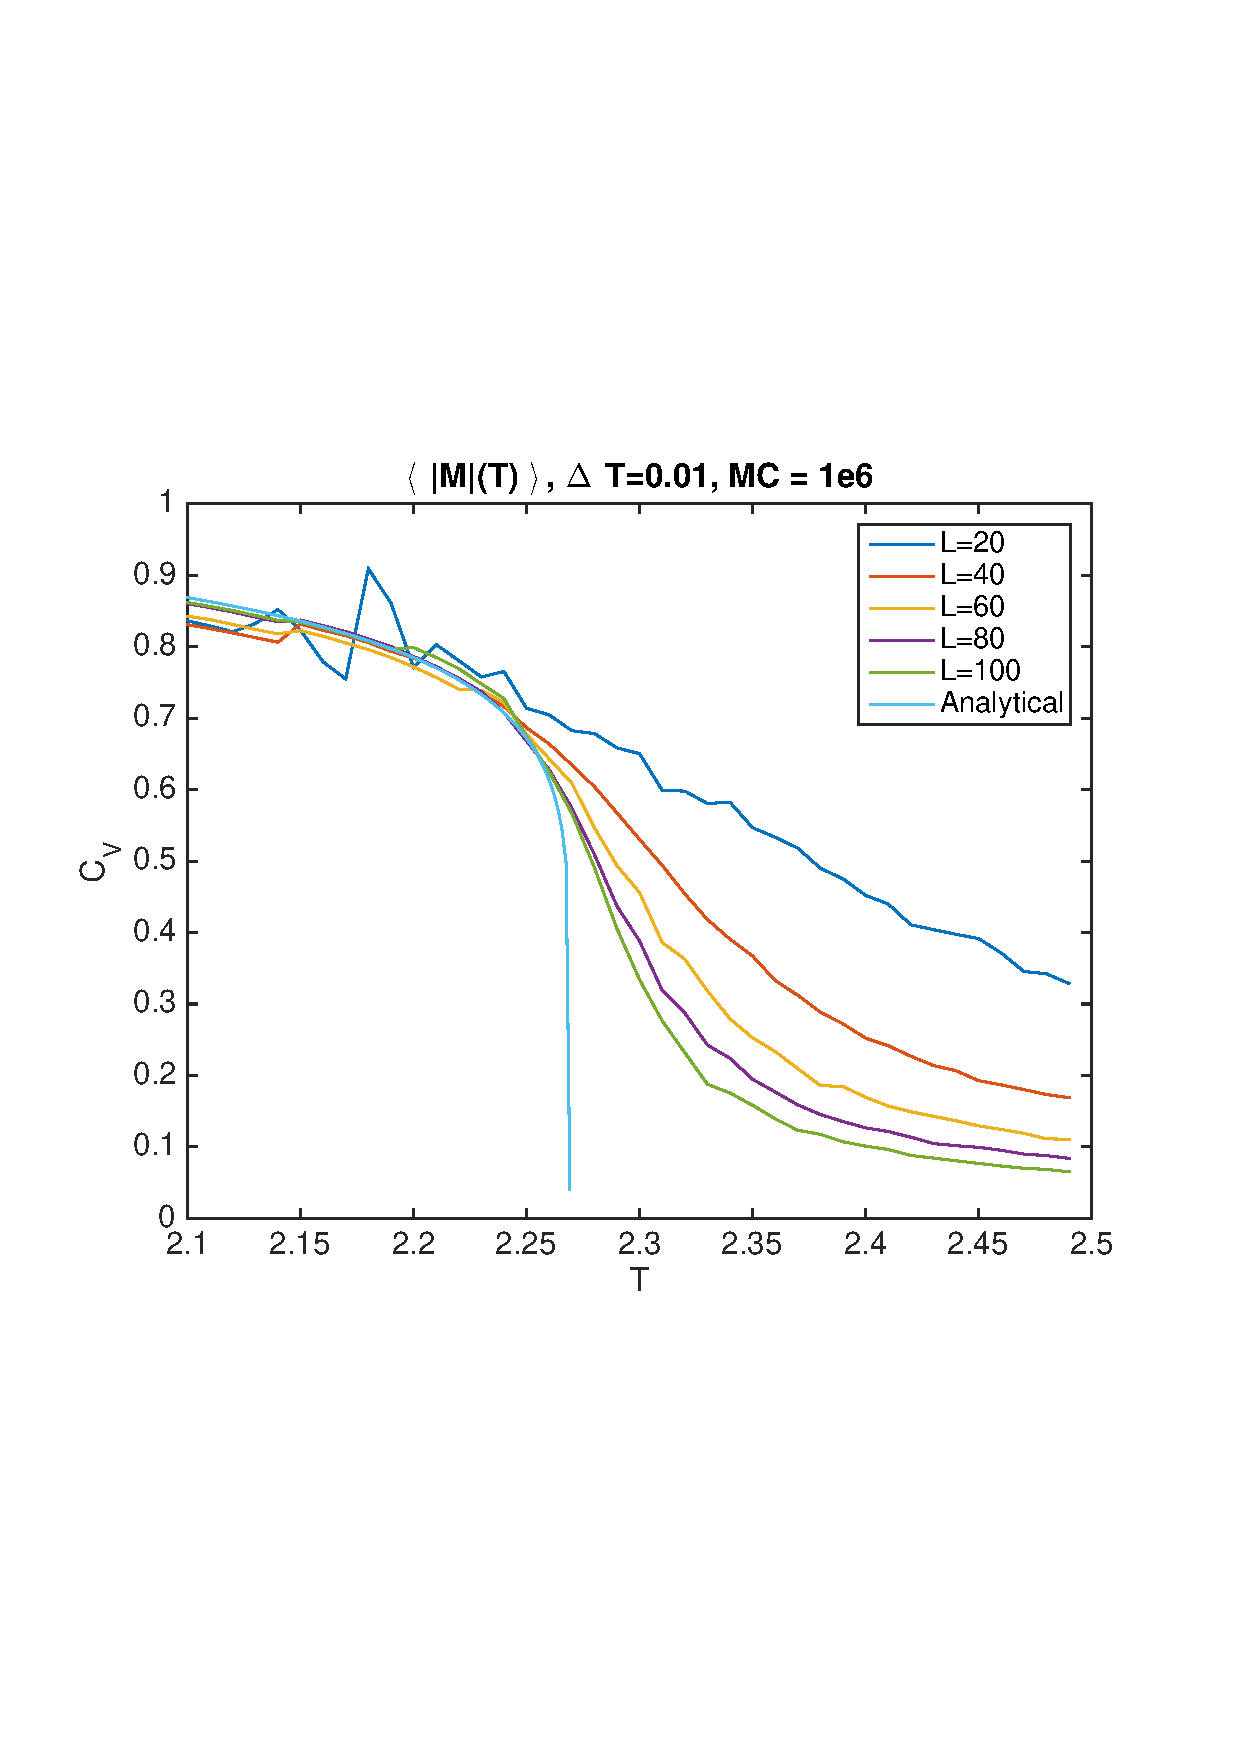
\includegraphics[scale = 0.6, trim = 1cm 8cm 1cm 8cm]{avg_mag_num_anal.pdf}
	\caption{Onsagers analytiske løsning er her plottet sammen med våre numeriske løsninger, vi ser at våre numeriske løsninger konvergerer fint mot den analytiske. Vi ser at over den kritiske temperaturen $T_C$ så har systemet null magnetisering.}
	\label{fig:avgmagnumanal}
\end{figure}

Det er også interessant å se på antall aksepterte tilstander som funksjon av MC-sykluser. I fig. (\ref{fig:AccStatesL20T1}) og (\ref{AccStatesL20T24}) ser vi hvordan systemet aksepterer nye tilstander ettersom syklusene går. Antallet aksepterte tilstander synker drastisk. Vi har plottet resultatet som aksepterte tilstander per antall MC-sykluser, og det er tydelig at for $T=2.4$ så skjer det mye oftere at nye tilstander blir akseptert enn for $T=1$. Dette kommer av at sistnevnte helst vil gå til en tilstand der alle spinn peker ned, mens førstnevnte har mer energi og vil gjerne mange spinn som peker opp også. Men begge systemene går mot null nye aksepterte tilstander når likevekt nås, dette skjer fordi systemet har lite å vinne på å akseptere nye tilstander siden det er i en tilstand som har ``perfekt'' energi i forhold til temperaturen vi har valgt.

\begin{figure}[H]
	\centering
	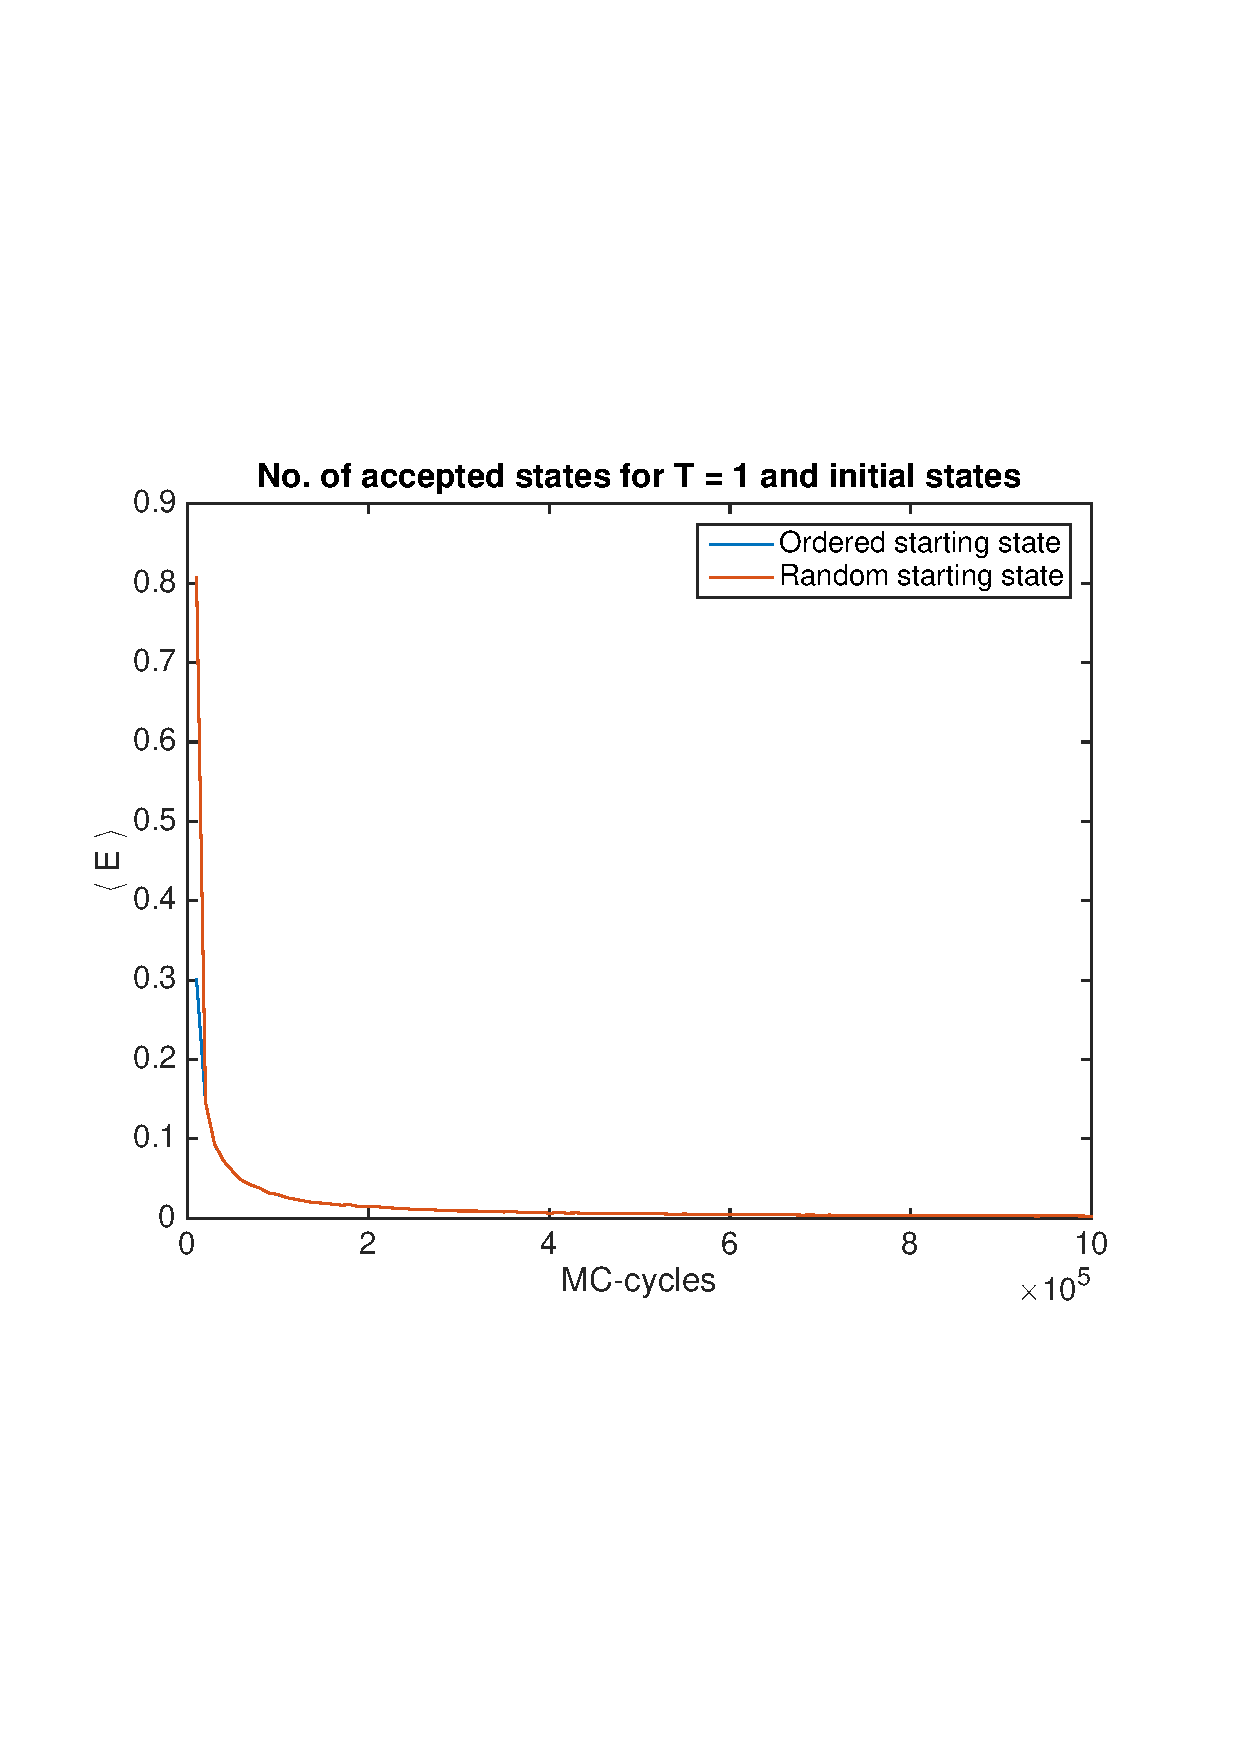
\includegraphics[scale = 0.6, trim = 1cm 8cm 1cm 8cm]{AccStatesL20T1.pdf}
	\caption{Antall aksepterte tilstander er alltid lavt for $T=1$ og går mot null når likevekt er nådd.}
	\label{fig:AccStatesL20T1}
\end{figure}

\begin{figure}[H]
	\centering
	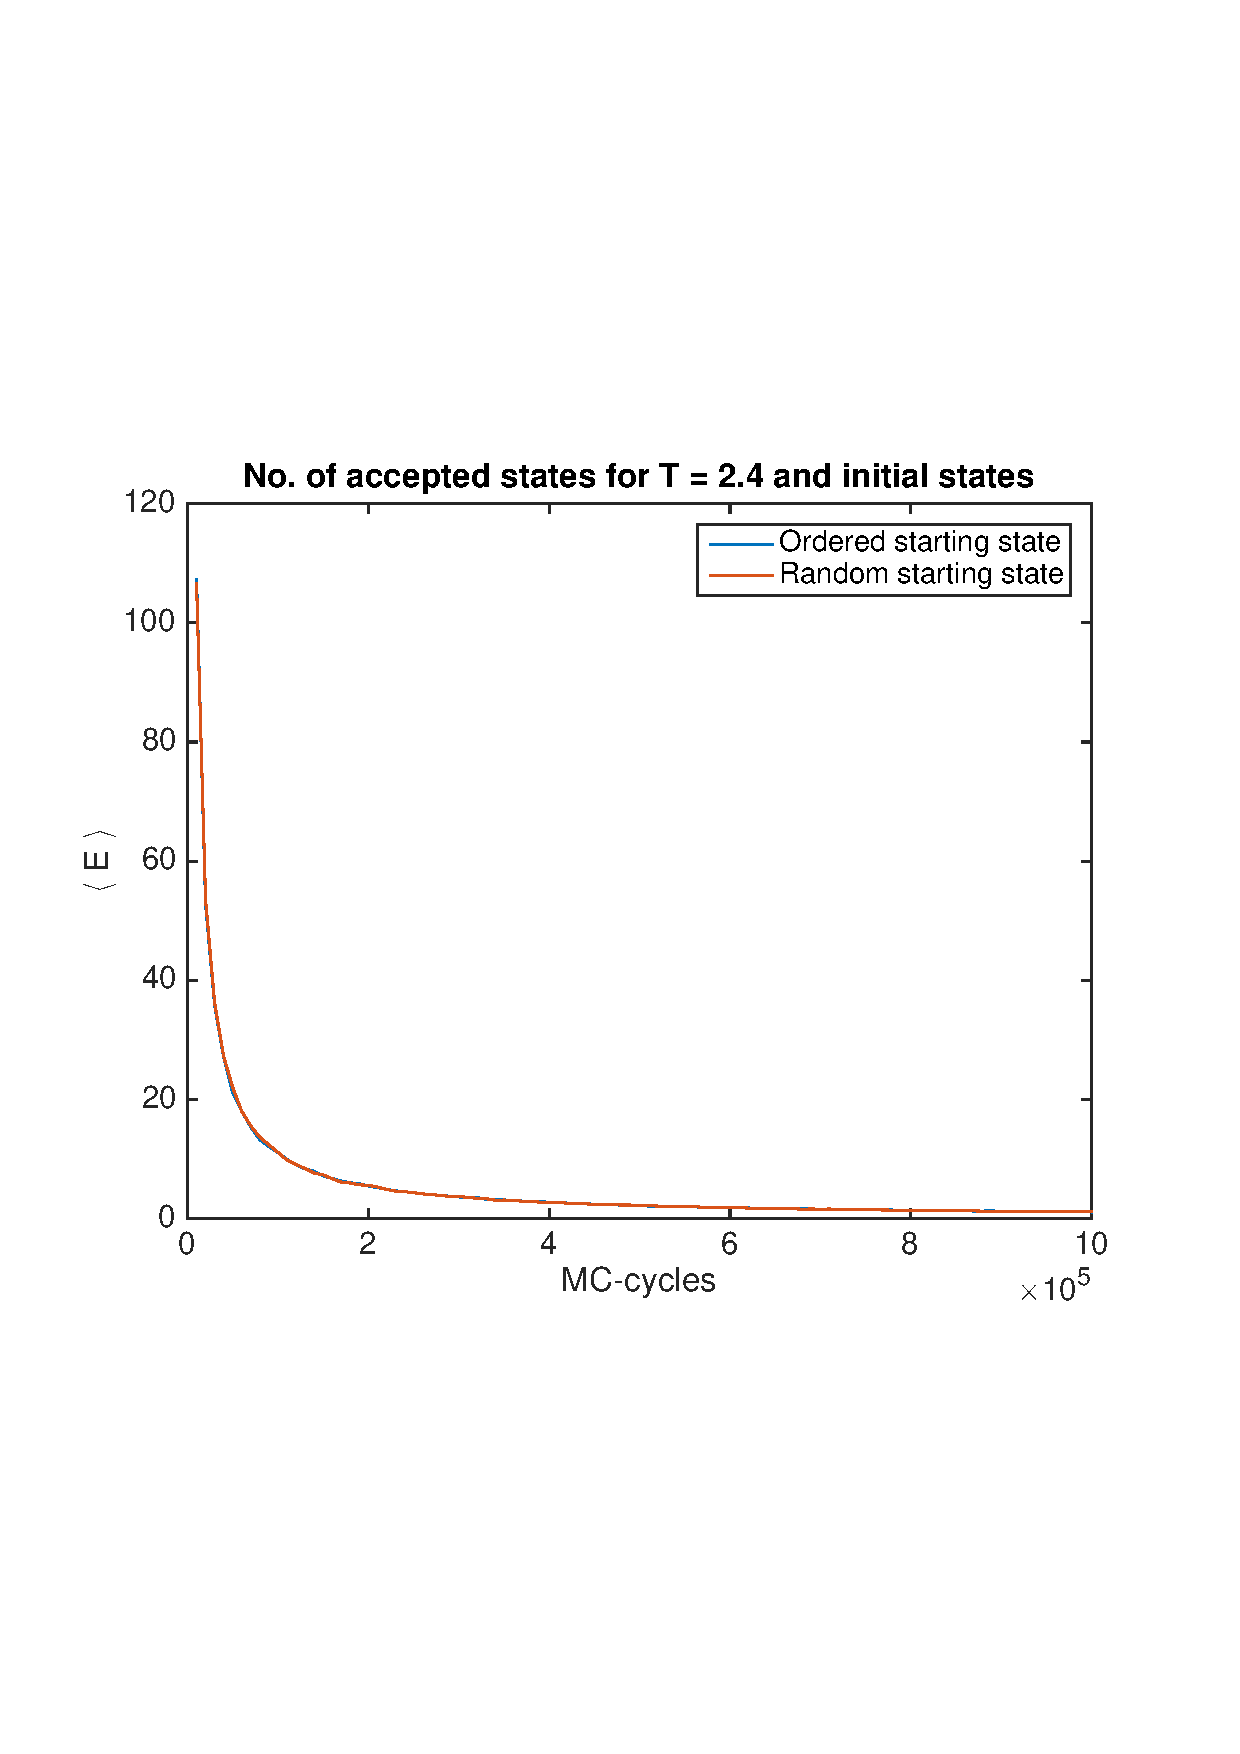
\includegraphics[scale = 0.6, trim = 1cm 8cm 1cm 8cm]{AccStatesL20T24.pdf}
	\caption{Setter vi $T=2.4$ aksepterer systemet mange nye tilstander og etter hvert også likevekt slik at antall aksepterte tilstander går mot null. Vi ser at starttilstand har ingenting å si, mens for $T=1$ så var det en liten forskjell i starten.}
	\label{fig:AccStatesL20T24}
\end{figure}


\begin{table}[H]
  \centering
  \begin{tabular}{ l l l l l}
    \toprule
    $I_{\text{Legendre}}$ & $I_{\text{Laguerre}}$ & $\epsilon_{\text{Legendre}}$ & $\epsilon_{\text{Laguerre}}$ & n \\
    \midrule
	0.129834 & 0.181567 & 0.326466 & 0.058093 & 10 \\
	0.199475 & 0.195887 & 0.034804 & 0.016192 & 15 \\
	0.177065 & 0.195636 & 0.081449 & 0.014892 & 20 \\
	0.189110 & 0.195240 & 0.018967 & 0.012837 & 25 \\
	0.185796 & 0.195070 & 0.036158 & 0.011955 & 30 \\
	\bottomrule
  \end{tabular}
  \caption{Resultat fra kjøringer av begge GK-metodene. Ingen av de er spesielt gode sammenliknet med Monte Carlo-metodene. Når vi hadde ti integrasjonspunkter så betydde det $10^6$ utregninger siden det var en seksdobbel løkke, en lite effektiv måte å angripe problemet på.}
  \label{tab:gauleg}
\end{table}


\subsection*{Konklusjon}

\end{document}